% Options for packages loaded elsewhere
\PassOptionsToPackage{unicode}{hyperref}
\PassOptionsToPackage{hyphens}{url}
\PassOptionsToPackage{dvipsnames,svgnames,x11names}{xcolor}
%
\documentclass[
  11pt,
]{article}
\usepackage{amsmath,amssymb}
\usepackage{iftex}
\ifPDFTeX
  \usepackage[T1]{fontenc}
  \usepackage[utf8]{inputenc}
  \usepackage{textcomp} % provide euro and other symbols
\else % if luatex or xetex
  \usepackage{unicode-math} % this also loads fontspec
  \defaultfontfeatures{Scale=MatchLowercase}
  \defaultfontfeatures[\rmfamily]{Ligatures=TeX,Scale=1}
\fi
\usepackage{lmodern}
\ifPDFTeX\else
  % xetex/luatex font selection
\fi
% Use upquote if available, for straight quotes in verbatim environments
\IfFileExists{upquote.sty}{\usepackage{upquote}}{}
\IfFileExists{microtype.sty}{% use microtype if available
  \usepackage[]{microtype}
  \UseMicrotypeSet[protrusion]{basicmath} % disable protrusion for tt fonts
}{}
\makeatletter
\@ifundefined{KOMAClassName}{% if non-KOMA class
  \IfFileExists{parskip.sty}{%
    \usepackage{parskip}
  }{% else
    \setlength{\parindent}{0pt}
    \setlength{\parskip}{6pt plus 2pt minus 1pt}}
}{% if KOMA class
  \KOMAoptions{parskip=half}}
\makeatother
\usepackage{xcolor}
\usepackage[margin=0.9in]{geometry}
\usepackage{longtable,booktabs,array}
\usepackage{calc} % for calculating minipage widths
% Correct order of tables after \paragraph or \subparagraph
\usepackage{etoolbox}
\makeatletter
\patchcmd\longtable{\par}{\if@noskipsec\mbox{}\fi\par}{}{}
\makeatother
% Allow footnotes in longtable head/foot
\IfFileExists{footnotehyper.sty}{\usepackage{footnotehyper}}{\usepackage{footnote}}
\makesavenoteenv{longtable}
\usepackage{graphicx}
\makeatletter
\def\maxwidth{\ifdim\Gin@nat@width>\linewidth\linewidth\else\Gin@nat@width\fi}
\def\maxheight{\ifdim\Gin@nat@height>\textheight\textheight\else\Gin@nat@height\fi}
\makeatother
% Scale images if necessary, so that they will not overflow the page
% margins by default, and it is still possible to overwrite the defaults
% using explicit options in \includegraphics[width, height, ...]{}
\setkeys{Gin}{width=\maxwidth,height=\maxheight,keepaspectratio}
% Set default figure placement to htbp
\makeatletter
\def\fps@figure{htbp}
\makeatother
\setlength{\emergencystretch}{3em} % prevent overfull lines
\providecommand{\tightlist}{%
  \setlength{\itemsep}{0pt}\setlength{\parskip}{0pt}}
\setcounter{secnumdepth}{5}
% definitions for citeproc citations
\NewDocumentCommand\citeproctext{}{}
\NewDocumentCommand\citeproc{mm}{%
  \begingroup\def\citeproctext{#2}\cite{#1}\endgroup}
\makeatletter
 % allow citations to break across lines
 \let\@cite@ofmt\@firstofone
 % avoid brackets around text for \cite:
 \def\@biblabel#1{}
 \def\@cite#1#2{{#1\if@tempswa , #2\fi}}
\makeatother
\newlength{\cslhangindent}
\setlength{\cslhangindent}{1.5em}
\newlength{\csllabelwidth}
\setlength{\csllabelwidth}{3em}
\newenvironment{CSLReferences}[2] % #1 hanging-indent, #2 entry-spacing
 {\begin{list}{}{%
  \setlength{\itemindent}{0pt}
  \setlength{\leftmargin}{0pt}
  \setlength{\parsep}{0pt}
  % turn on hanging indent if param 1 is 1
  \ifodd #1
   \setlength{\leftmargin}{\cslhangindent}
   \setlength{\itemindent}{-1\cslhangindent}
  \fi
  % set entry spacing
  \setlength{\itemsep}{#2\baselineskip}}}
 {\end{list}}
\usepackage{calc}
\newcommand{\CSLBlock}[1]{\hfill\break\parbox[t]{\linewidth}{\strut\ignorespaces#1\strut}}
\newcommand{\CSLLeftMargin}[1]{\parbox[t]{\csllabelwidth}{\strut#1\strut}}
\newcommand{\CSLRightInline}[1]{\parbox[t]{\linewidth - \csllabelwidth}{\strut#1\strut}}
\newcommand{\CSLIndent}[1]{\hspace{\cslhangindent}#1}
\ifLuaTeX
\usepackage[bidi=basic]{babel}
\else
\usepackage[bidi=default]{babel}
\fi
\babelprovide[main,import]{american}
% get rid of language-specific shorthands (see #6817):
\let\LanguageShortHands\languageshorthands
\def\languageshorthands#1{}
\usepackage[dvipsnames]{xcolor}
\usepackage{microtype}
\usepackage{caption}
\usepackage{placeins}
\usepackage{float}
\floatplacement{figure}{H}
\captionsetup{font=small,labelfont=bf}
\setlength{\emergencystretch}{3em}
\raggedbottom
\AtBeginDocument{\hypersetup{pdfauthor={Human authorship and review TBD},pdfsubject={Exploratory expanded channeling study; model-agent review, not human peer review}}}
\ifLuaTeX
  \usepackage{selnolig}  % disable illegal ligatures
\fi
\usepackage{bookmark}
\IfFileExists{xurl.sty}{\usepackage{xurl}}{} % add URL line breaks if available
\urlstyle{same}
\hypersetup{
  pdftitle={Comparing Named Claims and Texts in Online Channeling},
  pdfauthor={Living research draft --- human authorship and review TBD},
  pdflang={en-US},
  colorlinks=true,
  linkcolor={MidnightBlue},
  filecolor={Maroon},
  citecolor={MidnightBlue},
  urlcolor={MidnightBlue},
  pdfcreator={LaTeX via pandoc}}

\title{Comparing Named Claims and Texts in Online Channeling}
\usepackage{etoolbox}
\makeatletter
\providecommand{\subtitle}[1]{% add subtitle to \maketitle
  \apptocmd{\@title}{\par {\large #1 \par}}{}{}
}
\makeatother
\subtitle{Source registers, topic structure, and a cross-medium message
pilot}
\author{Living research draft --- human authorship and review TBD}
\date{8 November 2026}

\begin{document}
\maketitle
\begin{abstract}
Online channeling archives attach extraterrestrial, angelic, historical
and religious names to communications attributed to human mediums.
Comparing those communications requires separating people, publisher
accounts, claimed speakers, broad civilization labels and the text
actually observed. This exploratory companion study links a typed
register containing 41 person records, 52 claimed-name records and 69
relationships to two separately fitted text collections: a joint corpus
of 292 accepted source-context units comprising 774,110 words, and a new
pilot of 20 publisher-attributed message bodies comprising 20,829 words
from four mediums and 11 comparison labels. The register supports 19
comparison groups, but only four have cross-medium text in the new
pilot. Joint clustering closely tracks source context (adjusted Rand
index 0.824), while fixed-length windows substantially reduce several
lexical similarities. In the new pilot, mean TF-IDF cosine is 0.03636
across 12 shared-label, cross-medium document pairs and 0.06588 across
49 different-label, within-medium pairs. Exact council-title masking
changes these means to 0.03648 and 0.06538. These dependent, purposively
selected comparisons are consistent with a substantial role for
publisher or medium vocabulary but do not identify a causal style
effect. Source reading also rejects the sole surviving heuristic
question-retrieval candidate as a false match. We release metadata,
typed relations, plots, review records and rebuildable paper artifacts,
retaining full copyrighted texts and media privately. The study concerns
published discourse; it does not authenticate claimed beings, equate
contemporary messages with a religion's doctrine, or estimate
supernatural truth.
\end{abstract}

\FloatBarrier

\section{Introduction}\label{introduction}

A channel account is not a medium, a medium can be associated with
several named sources, and a shared name can refer to different claims
in different publishing contexts. These distinctions become
consequential when an online archive combines a historical dialogue
collection, recent interviews, promotional excerpts, publisher
transcripts and messages presented as coming from extraterrestrial
collectives or sacred figures. An attractive network can obscure those
differences if every account becomes a person, every mention becomes a
speaker attribution, or every shared word becomes evidence of agreement.

This study expands an existing Bashar--Ra source project while
preserving its earlier analyses and paper. The expansion follows
user-selected channel accounts and a bounded set of publisher-linked
leads. It asks how a larger comparison can remain auditable when
available evidence ranges from a readable message body to a directory
listing, a channel biography or an inaccessible archive page. The
practical objective is a research dashboard and living paper in which a
reader can move from a group comparison to a person, an attributed
source, an actual document and its collection status.

The unit of analysis matters. ``Pleiadian'' can label a civilization, a
named council, an unnamed collective or a particular attributed speaker.
``Kryon'' is a named entity label, not a civilization. A publisher's
``Hathors'' collective should not automatically become the Egyptian
goddess Hathor. A claimed modern message labeled ``Ra'' should not be
silently combined with the historical L/L Research material or with an
Egyptian religious tradition. Similarly, a host introducing a guest, a
researcher maintaining an archive and a reposter publishing excerpts are
not additional mediums by virtue of appearing on a channel.

Our contribution is an integrated comparison protocol and an executed,
bounded example. The protocol preserves typed attribution and unresolved
identity, separates the source register from observed text,
distinguishes lexical retrieval from equivalent questions, and binds
published figures to immutable inputs. The empirical work combines a new
joint fit of accepted texts with a small, separately analyzed message
pilot. It adds evidence about this corpus and its measurement problems;
it does not introduce a new topic-model algorithm or claim to be the
first computational study of religion, channeling or online video.

Three questions guide the paper:

\begin{enumerate}
\def\labelenumi{\arabic{enumi}.}
\tightlist
\item
  \textbf{Attribution and coverage:} Which repeated labels have multiple
  directly attributed human records, and which have enough observed
  cross-medium text to support comparison?
\item
  \textbf{Lexical organization:} How do source-context similarity,
  exploratory topics and clusters change with length, genre and
  name-masking controls?
\item
  \textbf{Interpretive validity:} Do lexical matches yield equivalent
  questions or comparable practical recommendations when their source
  contexts are read?
\end{enumerate}

These are exploratory questions, not preregistered hypotheses. The
manuscript is an AI-assisted living research draft. Human authorship,
independent human annotation and external peer review remain TBD.

\FloatBarrier

\section{Methodological context}\label{methodological-context}

A source-rich archive can still be a poor basis for inference if
curation, speaker roles, language, editing and recording conditions are
unspecified. Data statements provide a useful framework for reporting
such decisions (\citeproc{ref-bender2018}{Bender and Friedman 2018}). We
apply that principle by distinguishing edited historical dialogue,
mixed-speaker ASR, publisher-hosted captions, PDF excerpts and
publisher-attributed message bodies. The same framework explains why an
account inventory cannot serve as a denominator for analyzed speech.

Topic models also require interpretation beyond their most prominent
words. Doogan and Buntine examine limits of aggregate interpretability
measures and motivate reading representative documents alongside topic
displays (\citeproc{ref-doogan2021}{Doogan and Buntine 2021}). Our
factor labels are therefore descriptive term lists, not discovered
doctrines. Their human expert evaluation was not reproduced here.
Schroeder and Wood-Doughty distinguish reliability questions from simple
similarity or stability diagnostics
(\citeproc{ref-schroeder2025}{Schroeder and Wood-Doughty 2025}). Their
experiments concern LDA; they do not validate our NMF settings or
provide a general threshold for meaningful cosine similarity. We report
our seed and perturbation checks by their actual scope.

Leakage and source dependence are relevant even when the immediate task
is unsupervised. Multiple excerpts from one recording, editions of one
session and text repeated by different accounts can exaggerate apparent
diversity. The abstract-level evidence inspected for Kapoor and
Narayanan motivates explicit provenance and caution about future
predictive claims (\citeproc{ref-kapoor2023}{Kapoor and Narayanan
2023}). It does not establish that the present corpus is free of
shared-source dependence. Any later classifier or language-model
evaluation should keep related recordings, excerpts and editions
together when separating training and evaluation data.

ASR introduces a different uncertainty. The abstract inspected for
Koenecke and colleagues documents hallucinated speech in its evaluated
conditions (\citeproc{ref-koenecke2024}{Koenecke et al. 2024}). We use
it to motivate preservation of audio provenance and a future listening
audit, not to import a hallucination rate into this collection. A
complete decoder pass proves that a retained file can be processed; it
does not establish recognition accuracy, speaker identity or
correspondence between a recording and a publisher transcript.

A substantive review of channeling and religious-studies scholarship,
together with YouTube and platform-study literature, remains
\textbf{TBD}. This methods-focused selection does not establish
scholarly novelty.

The five methodological references were inspected in an earlier project
increment at the access depths documented in Appendix A. This companion
paper reuses that record. It does not claim a fresh, comprehensive
literature review, a new review of entire papers whose abstracts alone
were available, or verified compliance with a current conference
submission template.

\FloatBarrier

\section{Source design and
collection}\label{source-design-and-collection}

\FloatBarrier

\subsection{Three evidence layers}\label{three-evidence-layers}

The register, the text corpus and the interpretation are separate
objects. The \textbf{register} stores attributed relationships: a person
reportedly channels a named entity or collective, works with a
civilization label, reports contact, appears in a series, or is merely
associated with an archive category. The \textbf{observed text}
comprises exact retained documents admitted under a stated extraction
rule. The \textbf{interpretation} is a bounded reading or exploratory
calculation grounded in those documents. No layer automatically supplies
the missing evidence required by another.

Source records include a canonical URL, actual access depth, retrieval
status, date, content or artifact hash and a supporting location or
paraphrase. Historical retained metadata remains historical. Failed
requests and rejected candidates remain in the ledger without becoming
supporting observations. A formerly relevant domain that now returns
unrelated material is not evidence for its historical claimant. The
graph merges shared person IDs only when immutable identity fields
agree; uncertain aliases and distinct source-specific labels remain
separate.

The typed graph contains \textbf{150 source records, 41 person records,
52 claimed-name records and 69 relations}. These include weaker
relationships and non-medium roles. They are not counts of authenticated
people, complete channels, independent origins or true paranormal
communications. Its \textbf{19 comparison groups} distinguish
civilization labels, shared names and related-name/aspect comparisons.
This last category matters, for example, when a publisher expressly
distinguishes a particular Magdalen aspect rather than claiming an
interchangeable source.

\begin{figure}
\centering
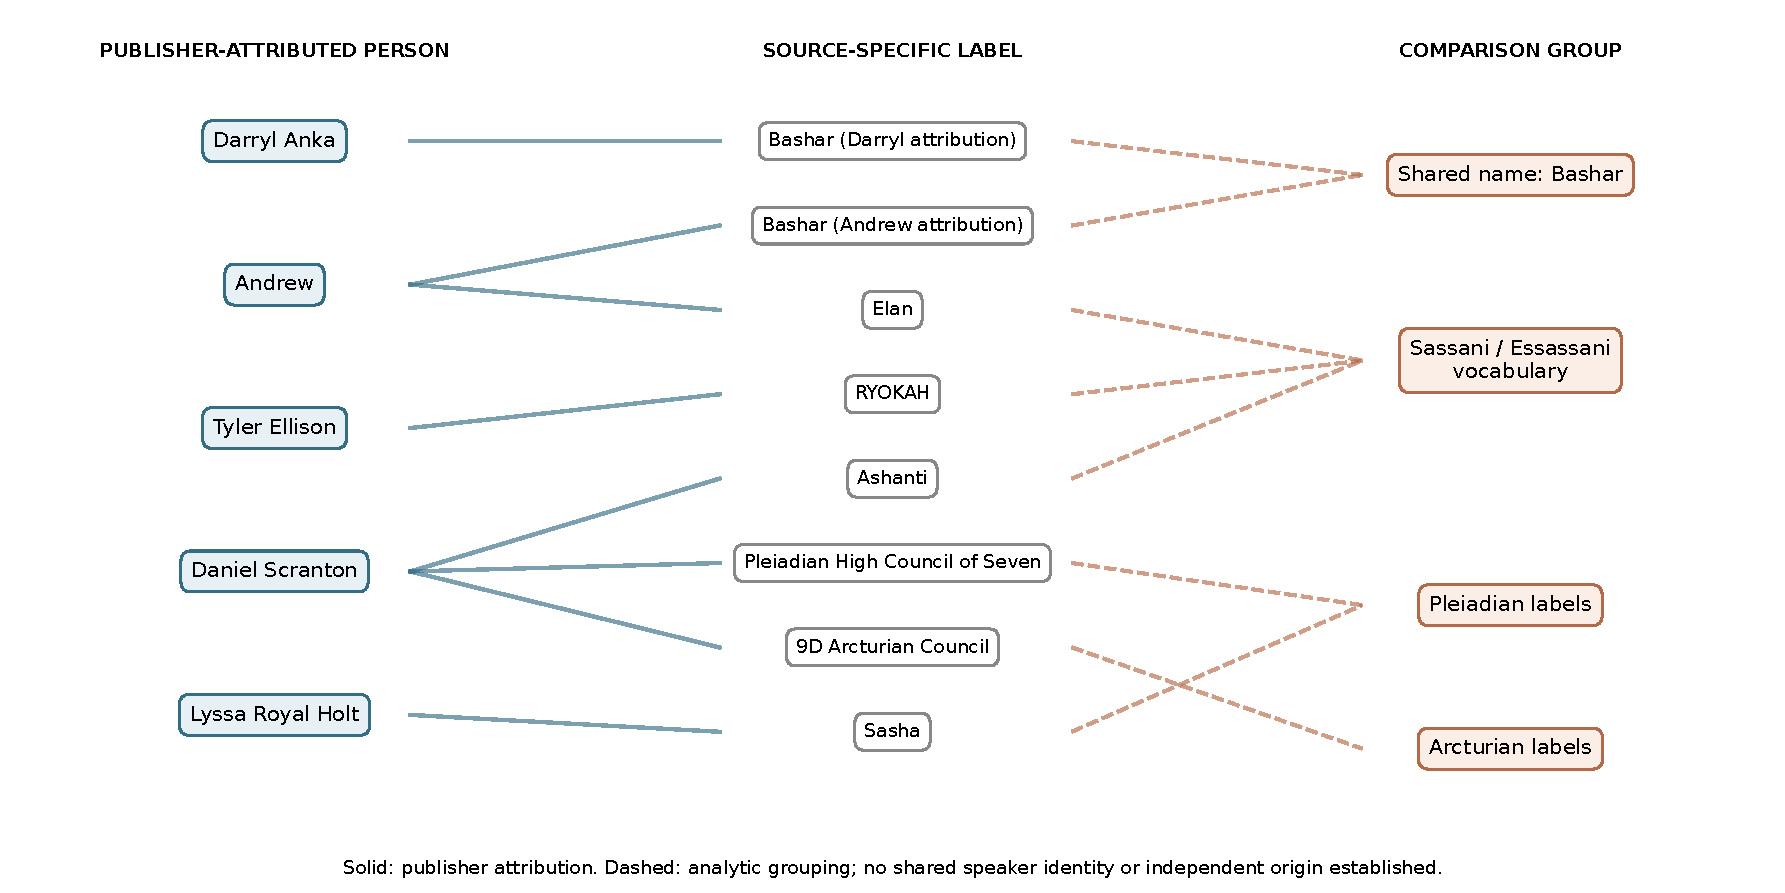
\includegraphics[width=1\textwidth,height=\textheight]{figures/typed-network-example.pdf}
\caption{An illustrative slice of the typed graph. Solid links encode
publisher attribution; dashed links encode a comparison grouping. The
two Bashar records remain source-specific. The diagram deliberately does
not place Bashar in a Sassani group without the required affiliation
evidence in this source frame.}
\end{figure}

\FloatBarrier

\subsection{Discovery, queries and
access}\label{discovery-queries-and-access}

Discovery began from the screened subscription accounts and inherited
repository leads, followed by ordinary public publisher pages and
first-page search-index results. Queries combined \emph{channeling} with
names and civilization labels, including Sassani, Ryokah, Royukh,
Pleiadians, Arcturians, Yahyel, Zeta, Andromedan, Ra, Kryon and Nine;
the complementary traditions work examined angelic, religious and
named-person claims. The registers preserve executed query strings and
source receipts. Ranked results were discovery aids rather than random
samples, body-level evidence or complete upload counts. Search-engine
summaries were not accepted as source assertions. Unrelated results and
unsuccessful requests were recorded rather than converted into evidence.

The user spelling \emph{Royukh} remains unresolved. RYOKAH and RYO
appear in Tyler Ellison's publisher branding, while other variants
appear in testimonials or indexed titles. A search engine returning a
plausible neighboring spelling is insufficient to assert an identity or
renaming history. Kristin Davies' inspected biography supports generic
mediumship claims but not an Erik attribution; the unsupported link was
excluded. Erik series metadata distinguishes the host from listed or
directly attributed mediums.

YouTube access remained restricted in the managed runtime. Publisher
websites, permitted public text, feeds and page-linked recordings
provided separate acquisition routes. No alternate egress or proxy-site
route was used to turn an inaccessible platform response into an
asserted crawl. The current duration policy admits non-Bashar recordings
without a five-minute threshold, while \textbf{Bashar material retains a
300-second minimum}. The earlier count cap is not retained. These rules
govern new collection; they do not retroactively make historical cohorts
complete.

A corrected parse of \textbf{23 saved Magenta publisher archive pages}
yielded \textbf{1,114 unique linked YouTube IDs}, including an
explicitly linked Short omitted by the earlier parser. This is
publisher-link metadata, not 1,114 downloaded videos, a verified
uploader-owned inventory or the total upload count. The separate new
audio frame comprises \textbf{224 RSS enclosures and five OmNa
page-linked recordings}. Its collection and ASR progress are operational
states with their own timestamps and receipts. We omit changing
completion counts from this fixed paper snapshot. The dashboard exposes
the current hash-bound projection separately.

\FloatBarrier

\subsection{The accepted joint corpus}\label{the-accepted-joint-corpus}

The joint fit admits accepted, normalized English text from three
previous study outputs, with exact-media or exact-text aliases already
collapsed under their recorded rules. It retains the earlier analyses
rather than overwriting them. Each admitted artifact is rechecked for
identity, bytes, hash and word count. Earlier full acquisition and ASR
validations are reused as prior evidence; the joint fit does not claim
that all media or speech recognition was performed again.

\begin{longtable}[]{@{}
  >{\raggedright\arraybackslash}p{(\columnwidth - 4\tabcolsep) * \real{0.6000}}
  >{\raggedright\arraybackslash}p{(\columnwidth - 4\tabcolsep) * \real{0.1600}}
  >{\raggedright\arraybackslash}p{(\columnwidth - 4\tabcolsep) * \real{0.2400}}@{}}
\caption{Accepted joint source-context units. Word counts are
whitespace-delimited after the stated normalization. Context labels do
not identify every speaker in a document.}\tabularnewline
\toprule\noalign{}
\begin{minipage}[b]{\linewidth}\raggedright
Source context
\end{minipage} & \begin{minipage}[b]{\linewidth}\raggedright
Units
\end{minipage} & \begin{minipage}[b]{\linewidth}\raggedright
Words
\end{minipage} \\
\midrule\noalign{}
\endfirsthead
\toprule\noalign{}
\begin{minipage}[b]{\linewidth}\raggedright
Source context
\end{minipage} & \begin{minipage}[b]{\linewidth}\raggedright
Units
\end{minipage} & \begin{minipage}[b]{\linewidth}\raggedright
Words
\end{minipage} \\
\midrule\noalign{}
\endhead
\bottomrule\noalign{}
\endlastfoot
Ra edited sessions & 106 & 278,601 \\
Bashar-related interviews / commentary & 19 & 222,699 \\
Official Bashar excerpts & 75 & 62,590 \\
Official promotion / product & 4 & 2,895 \\
Official greetings & 3 & 2,051 \\
Tracy publisher captions & 70 & 144,568 \\
Magenta transcript PDFs & 15 & 60,706 \\
Total & 292 & 774,110 \\
\end{longtable}

The 292 units are not 292 independently sampled recordings or verified
channeling sessions. Ra pages are edited published sessions. The
Bashar-related interviews and commentary contain mixed voices;
official-channel origin does not identify every utterance in an excerpt,
greeting or promotional item. The Tracy captions and Magenta PDFs also
retain their own publisher and extraction limitations. Reference works,
incomplete handouts, excluded language editions and alias dispositions
remain recorded separately.

\begin{figure}
\centering
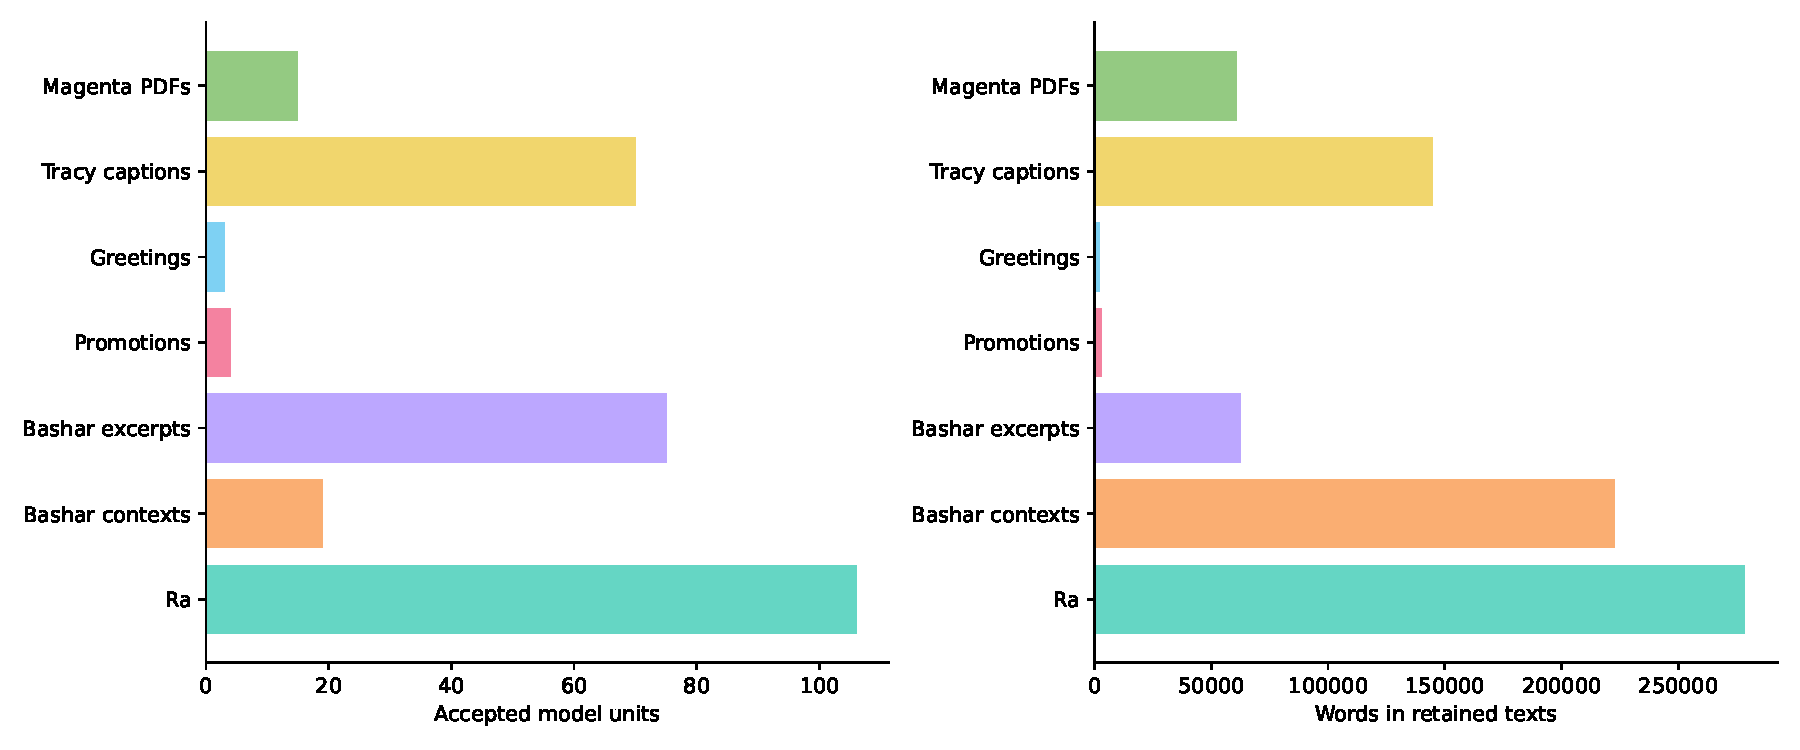
\includegraphics[width=0.92\textwidth,height=\textheight]{figures/joint-coverage.pdf}
\caption{Joint corpus coverage by source context. The unequal number and
length of observed units are properties of the selected source frame,
not prevalence estimates for the broader channeling ecosystem.}
\end{figure}

\FloatBarrier

\subsection{The new attributed-message
pilot}\label{the-new-attributed-message-pilot}

The second fit contains \textbf{20 newly collected message bodies,
20,829 words, four mediums and 11 comparison labels}. It is a purposive
feasibility sample with explicit page-local attribution and extraction
boundaries. It is neither a complete archive nor a random sample. The
four contexts and their sizes are shown below.

\begin{longtable}[]{@{}
  >{\raggedright\arraybackslash}p{(\columnwidth - 6\tabcolsep) * \real{0.4300}}
  >{\raggedright\arraybackslash}p{(\columnwidth - 6\tabcolsep) * \real{0.1600}}
  >{\raggedright\arraybackslash}p{(\columnwidth - 6\tabcolsep) * \real{0.1800}}
  >{\raggedright\arraybackslash}p{(\columnwidth - 6\tabcolsep) * \real{0.2300}}@{}}
\caption{New message pilot. The label sets overlap across mediums; their
row counts therefore do not sum to the 11 unique comparison
labels.}\tabularnewline
\toprule\noalign{}
\begin{minipage}[b]{\linewidth}\raggedright
Publisher-attributed medium
\end{minipage} & \begin{minipage}[b]{\linewidth}\raggedright
Documents
\end{minipage} & \begin{minipage}[b]{\linewidth}\raggedright
Words
\end{minipage} & \begin{minipage}[b]{\linewidth}\raggedright
Distinct comparison labels
\end{minipage} \\
\midrule\noalign{}
\endfirsthead
\toprule\noalign{}
\begin{minipage}[b]{\linewidth}\raggedright
Publisher-attributed medium
\end{minipage} & \begin{minipage}[b]{\linewidth}\raggedright
Documents
\end{minipage} & \begin{minipage}[b]{\linewidth}\raggedright
Words
\end{minipage} & \begin{minipage}[b]{\linewidth}\raggedright
Distinct comparison labels
\end{minipage} \\
\midrule\noalign{}
\endhead
\bottomrule\noalign{}
\endlastfoot
Daniel Scranton & 7 & 3,907 & 3 \\
Lyssa Royal Holt & 1 & 2,671 & 1 \\
Pamela Rose Kribbe & 4 & 7,324 & 4 \\
Natalie Glasson & 8 & 6,927 & 8 \\
\end{longtable}

Daniel Scranton's public WordPress responses illustrate the need for
body-level attribution. A keyword search for \emph{Pleiadian} returned
Arcturian messages containing incidental Pleiadian mentions or
promotional links. Only the actual message title and opening/closing
attribution determined the admitted label. Seven Daniel bodies were
bounded by the message paragraphs before promotional tails. The three
Pleiadian High Council messages were published in April 2016; the
Arcturian and Ashanti messages were published in 2026.

Lyssa Royal Holt's \emph{Preparedness} PDF is a five-page excerpt from a
session dated 23 July 1993. Its header identifies Sasha through Lyssa
Royal, and its body explicitly describes Sasha's own Pleiadian
community. The complete normalized dialogue contains 2,742 words. Five
printed \texttt{Question:} paragraphs were retained separately, while a
2,671-word response derivative entered the pilot. Continuation
attribution follows the printed layout; it is not a verified voice
identification. The excerpt is not represented as the complete
underlying recording or session.

Natalie Glasson and Pamela Rose Kribbe contribute messages with
page-local named attribution, including the two Marian name comparisons.
Publisher comments, navigation and unrelated material were excluded.
These modern messages are contemporary source claims, not representative
samples of Christianity, Buddhism, Hinduism, ancient Egyptian religion
or any other tradition whose names appear in the wider register. No
audio alignment of the 20 bodies was verified in this pilot.

\FloatBarrier

\section{Analysis}\label{analysis}

\FloatBarrier

\subsection{Lexical representations and
comparisons}\label{lexical-representations-and-comparisons}

Unicode compatibility normalization and tokenization preserve
apostrophes and negation. Complete source-name tokens are masked; the
procedure does not remove \texttt{don} from
\texttt{don\textquotesingle{}t} or \texttt{ll} from
\texttt{we\textquotesingle{}ll}. A declared filler list and English stop
list are used while retaining no, not, nor and never. This is a
specified token mask, not a guarantee that every source-identifying
phrase has disappeared.

For the joint study, TF-IDF uses unigrams and bigrams, sublinear term
frequency, smoothed inverse document frequency, L2 normalization, a
minimum document frequency of two and at most 12,000 features. Before
normalization, a term with positive count \(c_{td}\) receives weight

\[w_{td}=(1+\log c_{td})\left[\log\frac{1+N}{1+\operatorname{df}(t)}+1\right].\]

Cosine is the dot product of the normalized vectors. We average all
eligible unordered pairs within a context, excluding self-pairs, and all
cross-context pairs between contexts. These pair averages are
descriptive. A document participates in many pairs, so pair counts are
not independent sample sizes.

The joint sensitivity selects a centered 600-token span before masking
and transforms it with the fixed whole-document vocabulary and IDF.
Shorter documents are excluded rather than padded. A genre restriction
excludes official promotions and greetings plus baseline
promotional/skeptical formats. A separate removal of the single longest
document refits vocabulary and IDF. These changes probe sensitivity to
some format and length differences; they do not isolate a causal length
effect or eliminate all contextual confounding.

The pilot uses the same broad representation family with minimum
document frequency one and a fixed-IDF centered \textbf{300-token}
comparison. Twenty exact text hashes are distinct. A later sensitivity
removes explicit full council-title phrases before the existing token
mask and refits vocabulary/IDF. The original scores and exploratory
models remain available rather than being replaced after inspecting the
sensitivity.

\FloatBarrier

\subsection{Topics, partitions and lexical
networks}\label{topics-partitions-and-lexical-networks}

NMF and KMeans explore joint values of \(k=2\) through \(8\) with seeds
11, 23 and 47. Four NMF components are displayed for readability,
without declaring four optimal. Component names are prominent terms;
normalized component weights are factors, not probabilities of a
doctrine or validated topic membership.

For the joint KMeans display, the selected \(k\) maximizes the seed-11
cosine silhouette across the tested values. Source-context labels do not
enter fitting or this selection. The adjusted Rand comparison with
source contexts is then reported as a descriptive diagnostic. SVD
provides a two-dimensional display, not a spatial map of belief or a
validated measurement of conceptual distance. The pilot declares three
components/clusters for its small exploratory display rather than
optimizing an inferential criterion.

Two networks remain distinct. The typed claim network encodes documented
relationships and comparison groups. A lexical network exposes the top
25 cross-context TF-IDF pairs in the joint corpus. Its edges are
retrieval relationships, not social ties, corroboration, causal
influence or authenticated agreement between claimed entities. Reporting
them together without their edge types would obscure their different
meanings.

\FloatBarrier

\subsection{Question retrieval and source
reading}\label{question-retrieval-and-source-reading}

The private Q/A database separates printed documentary pairs from
unknown-speaker punctuation candidates. It contains 2,523 Ra pairs,
including four missing-question placeholders. A printed response is a
documentary pairing, not voice authentication. For other contexts,
punctuation is segmented within existing cue/page boundaries. An
adjacent fragment is not automatically an answer, and unknown answers
remain unknown.

Initial inspection exposed generic-fragment false matches. The corrected
exploratory retrieval requires 6--80 masked tokens and at least four
distinct non-stop content unigrams, uses question-only TF-IDF with
minimum document frequency one, and deduplicates exact question text
when fitting vocabulary. A candidate needs cosine at least 0.35, a
best-versus-runner-up margin at least 0.03 and at least three shared
content unigrams to become a review lead. Thresholds were adapted after
inspection; no precision estimate or held-out validation is claimed.

For the new pilot, the methods role read nine complete bounded bodies
totaling 11,274 primary words, plus the 71 Lyssa question words excluded
from its model text. Four comparative readings preserve shared themes,
different recommendations and counterexamples. The question headings
used to organize these readings were composed by the analyst. They are
not evidence that multiple mediums answered the same observed audience
question.

\FloatBarrier

\section{Results}\label{results}

\FloatBarrier

\subsection{Repeated labels are more common than comparable
text}\label{repeated-labels-are-more-common-than-comparable-text}

Thirteen of the 19 graph groups contain at least two directly attributed
human records. Only four have cross-medium message bodies in the new
pilot: Pleiadian labels, Arcturian labels, Mother Mary and Mary
Magdalene. The Pleiadian group has 11 direct-attribution human records
but 10 declared practices because Pia Orleane and Cullen Baird Smith
form a joint practice. Neither the person count nor the practice count
establishes independent origin.

\begin{longtable}[]{@{}
  >{\raggedright\arraybackslash}p{(\columnwidth - 6\tabcolsep) * \real{0.1800}}
  >{\raggedright\arraybackslash}p{(\columnwidth - 6\tabcolsep) * \real{0.5200}}
  >{\raggedright\arraybackslash}p{(\columnwidth - 6\tabcolsep) * \real{0.1400}}
  >{\raggedright\arraybackslash}p{(\columnwidth - 6\tabcolsep) * \real{0.1600}}@{}}
\caption{Selected repeated-label groups. ``Direct'' means an explicitly
supported attribution relationship, not paranormal verification or a
reviewed recording. Names may denote different councils, individuals or
aspects; their source-specific records remain separate.}\tabularnewline
\toprule\noalign{}
\begin{minipage}[b]{\linewidth}\raggedright
Comparison group
\end{minipage} & \begin{minipage}[b]{\linewidth}\raggedright
Direct-attribution people
\end{minipage} & \begin{minipage}[b]{\linewidth}\raggedright
Direct records
\end{minipage} & \begin{minipage}[b]{\linewidth}\raggedright
Pilot mediums
\end{minipage} \\
\midrule\noalign{}
\endfirsthead
\toprule\noalign{}
\begin{minipage}[b]{\linewidth}\raggedright
Comparison group
\end{minipage} & \begin{minipage}[b]{\linewidth}\raggedright
Direct-attribution people
\end{minipage} & \begin{minipage}[b]{\linewidth}\raggedright
Direct records
\end{minipage} & \begin{minipage}[b]{\linewidth}\raggedright
Pilot mediums
\end{minipage} \\
\midrule\noalign{}
\endhead
\bottomrule\noalign{}
\endlastfoot
Pleiadian labels & Arkayla, Barbara Marciniak, Cullen Baird Smith,
Daniel Scranton, Lyssa Royal Holt, Nora Herold, Pia Orleane, Rob
Gauthier, Sam the Illusionist, Wendy Kennedy, Natalie Glasson & 11 &
3 \\
Arcturian labels & Daniel Scranton, Natalie Glasson & 2 & 2 \\
Yahyel labels & Shaun Swanson, Wieteke Koolhof & 2 & 0 \\
Bashar & Andrew, Darryl Anka & 2 & 0 \\
Sassani / Essassani vocabulary & Andrew, Daniel Scranton, Tyler Ellison
& 3 & 1 \\
Archangel Michael & Daniel Scranton, Diana Muenz Chen, Natalie Glasson,
Ronna Herman Vezane & 4 & 1 \\
Mother Mary & Natalie Glasson, Pamela Rose Kribbe & 2 & 2 \\
Mary Magdalene / Magdalen & Natalie Glasson, Pamela Rose Kribbe, Tom
Kenyon & 3 & 2 \\
\end{longtable}

The repeated Bashar-name case requires careful wording.\footnote{Publisher
  source: \href{https://www.elaninteractions.com/about.html}{Elan
  Interactions, About}, inspected 8 November 2026. This is the
  publisher's training narrative.} Elan Interactions states that Bashar
trained Andrew for two years and that Darryl Anka confirmed this. The
inspected passage does not establish a direct human Andrew--Darryl
teacher relationship. It also makes an assumption of independent source
origin inappropriate. Andrew is identified by the first name used by the
publisher; an unverified expanded identity is not substituted.

Kryon and Ra each retain a directly attributed historical or established
publisher record alongside weaker modern archive-category evidence in
the wider register. A category association cannot be promoted to an
inspected session. The Erik group similarly distinguishes direct
attribution from people listed in series metadata. The current graph
therefore supports a research queue rather than a pretense that all
named-label comparisons already have equivalent evidence.

\begin{figure}
\centering
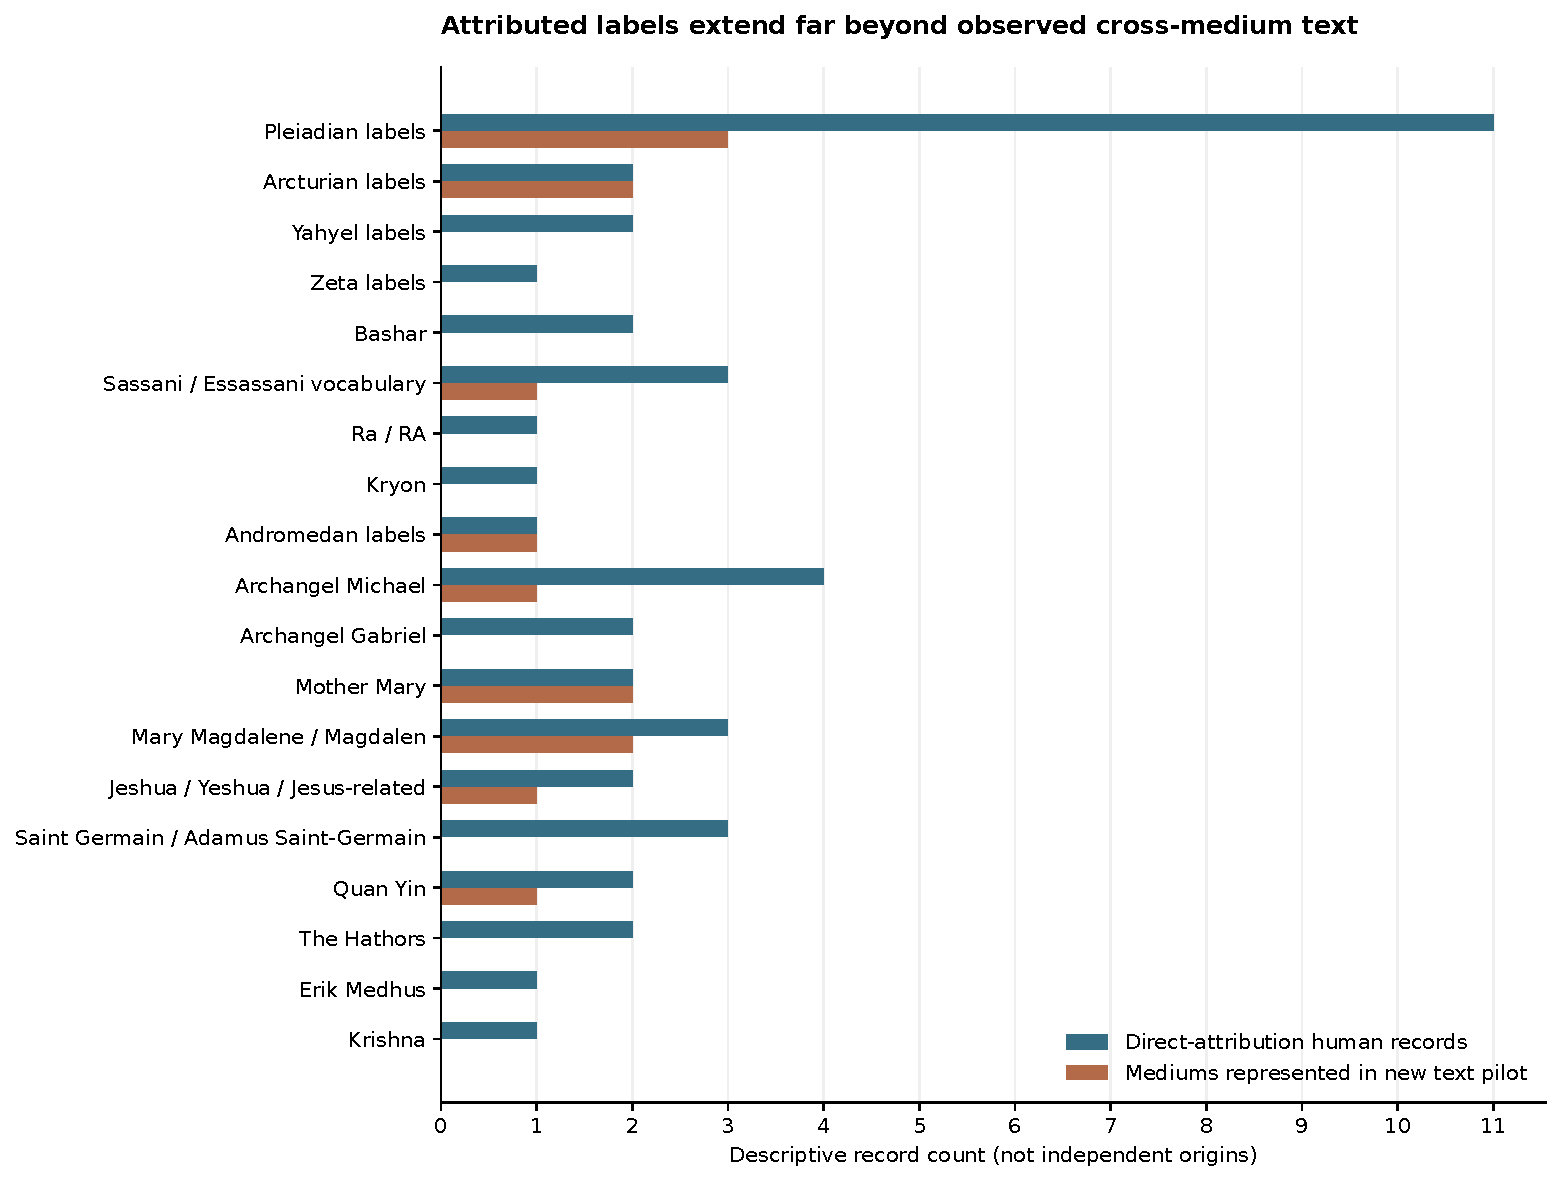
\includegraphics[width=0.96\textwidth,height=\textheight]{figures/claim-coverage.pdf}
\caption{Coverage gaps across all 19 comparison groups. Bars count
attributed human records and mediums represented in the new pilot. A
missing pilot bar means no admitted message in that frame, not no
message anywhere or zero similarity.}
\end{figure}

\FloatBarrier

\subsection{Joint lexical structure follows source
context}\label{joint-lexical-structure-follows-source-context}

The selected joint KMeans partition has \(k=3\), cosine silhouette
\textbf{0.08368} and source-context adjusted Rand index
\textbf{0.82384}. The close correspondence with source context is
evidence of substantial source organization in these vectors. It is not
validation of three underlying doctrines, nor a test of whether any
claimed entity exists. The relatively low silhouette and the dependence
on the tested representation further discourage a strong categorical
interpretation.

The four displayed NMF factors also align strongly with publishing
contexts. One emphasizes \emph{complex, entity, correct, density} and
receives a mean normalized weight of 0.905 in Ra sessions. Another
emphasizes \emph{soul, ascension, frequencies} and receives 0.881 in
Tracy captions. The \emph{idea, don't, not, reality} factor receives
0.922 in official Bashar excerpts. A \emph{starseeds, template,
energetic} factor receives 0.926 in Magenta PDFs. These are
group-average factor weights, not probabilities or externally validated
labels. Surviving source-specific expressions, editorial form and the
selection frame can contribute to this separation.

\begin{figure}
\centering
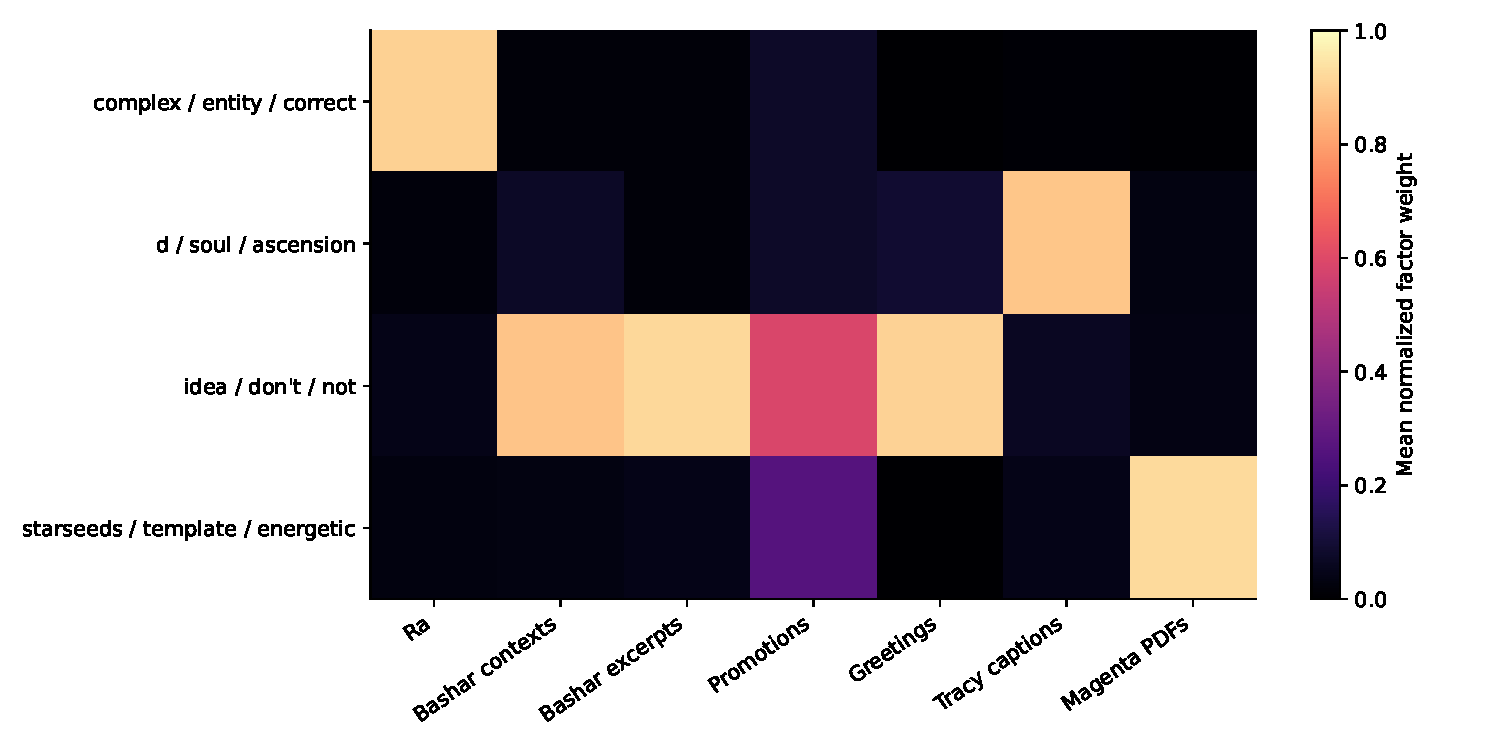
\includegraphics[width=1\textwidth,height=\textheight]{figures/joint-topics.pdf}
\caption{Four exploratory NMF components in the joint corpus. Top terms
summarize fitted factors; their source concentration is a reason to
examine provenance and genre, not to infer distinct extraterrestrial
doctrines.}
\end{figure}

Whole-document and centered-window similarities differ substantially.
The window analysis includes \textbf{278 of the 292 units}; 14 shorter
units are excluded. Selected comparisons make the scale of the change
explicit.

\begin{longtable}[]{@{}
  >{\raggedright\arraybackslash}p{(\columnwidth - 6\tabcolsep) * \real{0.4000}}
  >{\raggedright\arraybackslash}p{(\columnwidth - 6\tabcolsep) * \real{0.1800}}
  >{\raggedright\arraybackslash}p{(\columnwidth - 6\tabcolsep) * \real{0.1800}}
  >{\raggedright\arraybackslash}p{(\columnwidth - 6\tabcolsep) * \real{0.2400}}@{}}
\caption{Mean joint TF-IDF cosine for selected context pairs. The window
representation keeps the whole-text vocabulary/IDF but changes text
extent and, for some pairs, eligible units. Pair values are
dependent.}\tabularnewline
\toprule\noalign{}
\begin{minipage}[b]{\linewidth}\raggedright
Context pair
\end{minipage} & \begin{minipage}[b]{\linewidth}\raggedright
Full text
\end{minipage} & \begin{minipage}[b]{\linewidth}\raggedright
600-token spans
\end{minipage} & \begin{minipage}[b]{\linewidth}\raggedright
Pair counts: full / window
\end{minipage} \\
\midrule\noalign{}
\endfirsthead
\toprule\noalign{}
\begin{minipage}[b]{\linewidth}\raggedright
Context pair
\end{minipage} & \begin{minipage}[b]{\linewidth}\raggedright
Full text
\end{minipage} & \begin{minipage}[b]{\linewidth}\raggedright
600-token spans
\end{minipage} & \begin{minipage}[b]{\linewidth}\raggedright
Pair counts: full / window
\end{minipage} \\
\midrule\noalign{}
\endhead
\bottomrule\noalign{}
\endlastfoot
Ra / Bashar-related context & 0.10278 & 0.02589 & 2,014 / 2,014 \\
Bashar-related / official excerpt & 0.12843 & 0.05728 & 1,425 / 1,197 \\
Ra / Magenta & 0.07716 & 0.03066 & 1,590 / 1,590 \\
Tracy / Magenta & 0.09267 & 0.04210 & 1,050 / 1,050 \\
\end{longtable}

\begin{figure}
\centering
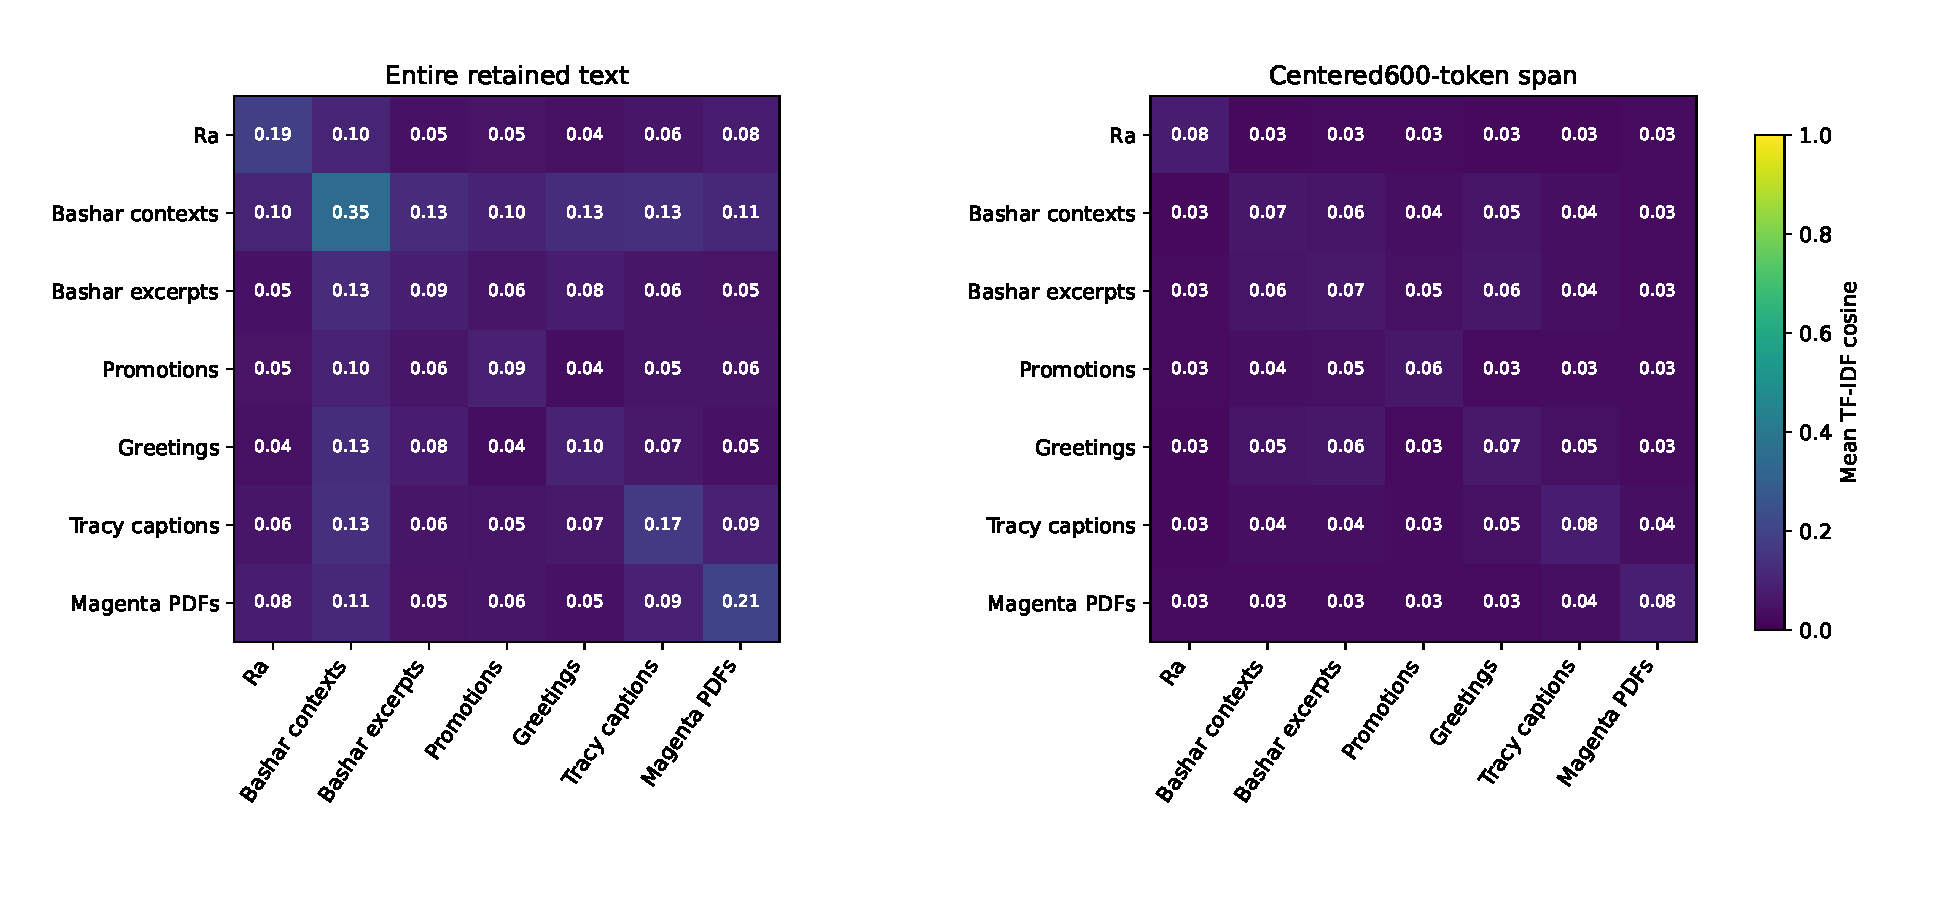
\includegraphics[width=1\textwidth,height=\textheight]{figures/joint-similarity.pdf}
\caption{Joint full-document and 600-token similarities. The figure
preserves the source-context grain and indicates a lexical comparison,
not source agreement.}
\end{figure}

The longest document is a Magenta PDF of \textbf{23,969 words}. It
appears in \textbf{19 of the 25} displayed cross-context lexical-network
edges. Removing that document and refitting reduces the Bashar-related
interview/Magenta mean from 0.11446 to 0.10479. This does not invalidate
the remaining links or prove a single length mechanism; it shows why a
visually central document should be inspected before a network is
interpreted as a convergence of independent sources.

The genre-restricted subset retains 284 units under the fixed
whole-corpus vocabulary and IDF, keeping the principal between-context
values close to their corresponding full-text estimates. For example, Ra
versus Bashar-related context changes from 0.10278 to 0.10222. That
limited change does not resolve the larger differences among edited
dialogue, spontaneous interviews, captions and handouts. A broad genre
exclusion is a sensitivity, not a matched design.

\begin{figure}
\centering
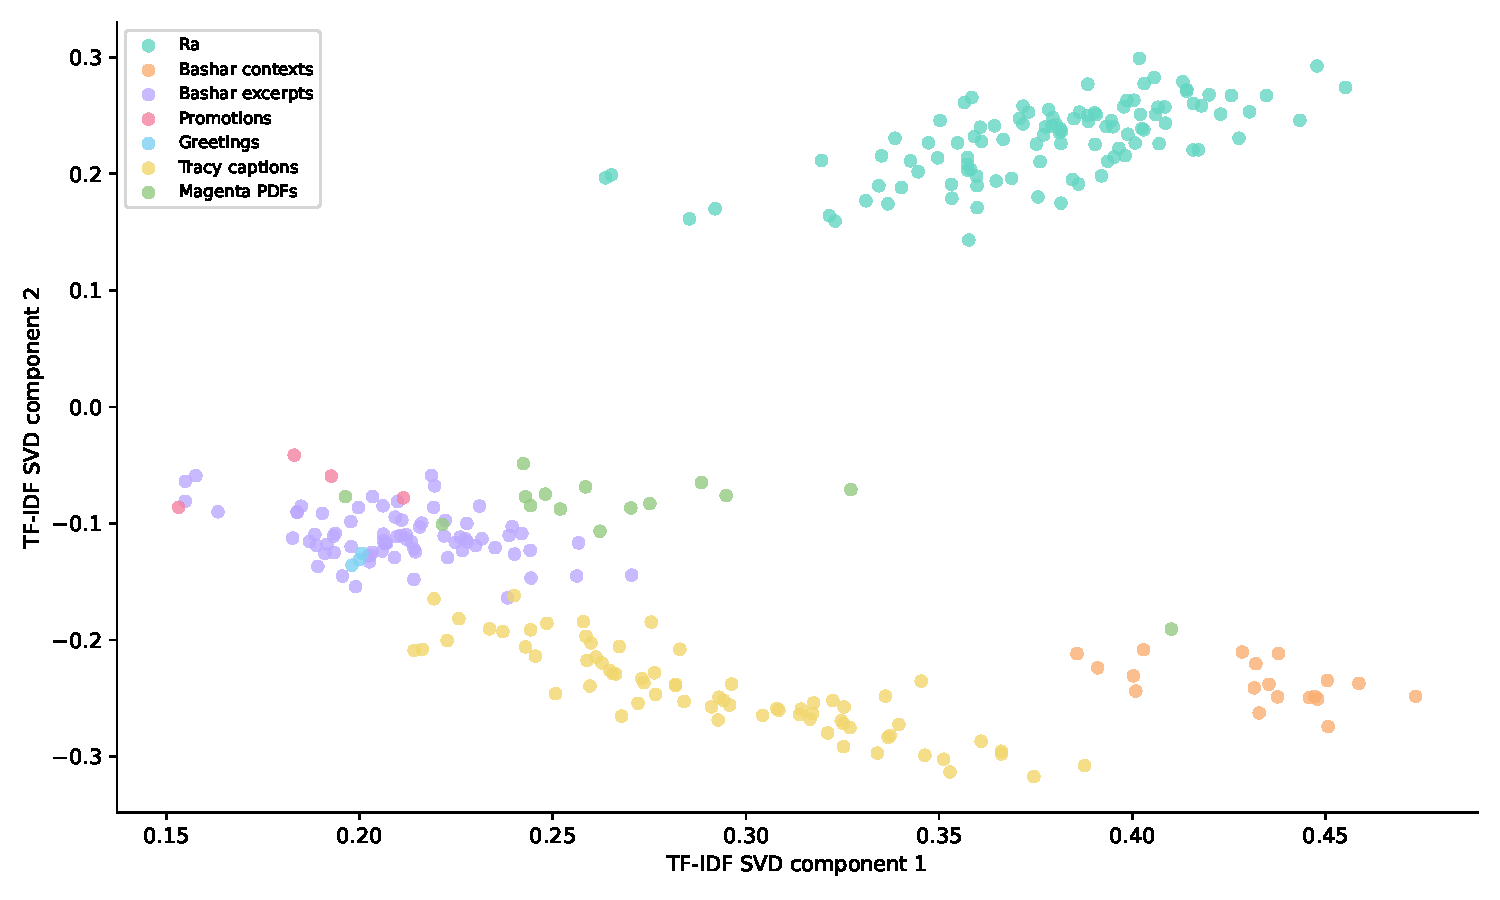
\includegraphics[width=0.92\textwidth,height=\textheight]{figures/joint-clusters.pdf}
\caption{SVD projection of joint TF-IDF vectors colored by source
context. The KMeans partition is evaluated separately. A two-dimensional
projection does not preserve every distance or establish independent
conceptual groups.}
\end{figure}

\FloatBarrier

\subsection{Shared-label pilot comparisons remain
heterogeneous}\label{shared-label-pilot-comparisons-remain-heterogeneous}

The 20-message pilot generates 190 unordered document pairs. Twelve are
shared-label comparisons across mediums: seven Pleiadian pairs, three
Arcturian pairs, one Mother Mary pair and one Mary Magdalene pair. The
first ten are \textbf{broad civilization-label} comparisons, not
comparisons of the same named personality. Forty-nine pairs compare
different labels within the same medium. The remaining 129 belong to
other pair configurations.

\begin{longtable}[]{@{}
  >{\raggedright\arraybackslash}p{(\columnwidth - 6\tabcolsep) * \real{0.4000}}
  >{\raggedright\arraybackslash}p{(\columnwidth - 6\tabcolsep) * \real{0.1800}}
  >{\raggedright\arraybackslash}p{(\columnwidth - 6\tabcolsep) * \real{0.1800}}
  >{\raggedright\arraybackslash}p{(\columnwidth - 6\tabcolsep) * \real{0.2400}}@{}}
\caption{Pilot pair averages. ``Other'' combines the remaining pair
configurations and is not a matched control group. All rows contain
dependent pairs, and no inferential test is reported.}\tabularnewline
\toprule\noalign{}
\begin{minipage}[b]{\linewidth}\raggedright
Pair configuration
\end{minipage} & \begin{minipage}[b]{\linewidth}\raggedright
Pairs
\end{minipage} & \begin{minipage}[b]{\linewidth}\raggedright
Full text
\end{minipage} & \begin{minipage}[b]{\linewidth}\raggedright
300-token spans
\end{minipage} \\
\midrule\noalign{}
\endfirsthead
\toprule\noalign{}
\begin{minipage}[b]{\linewidth}\raggedright
Pair configuration
\end{minipage} & \begin{minipage}[b]{\linewidth}\raggedright
Pairs
\end{minipage} & \begin{minipage}[b]{\linewidth}\raggedright
Full text
\end{minipage} & \begin{minipage}[b]{\linewidth}\raggedright
300-token spans
\end{minipage} \\
\midrule\noalign{}
\endhead
\bottomrule\noalign{}
\endlastfoot
Different label, same medium & 49 & 0.06588 & 0.03145 \\
Other configurations & 129 & 0.03730 & 0.01686 \\
Same label, cross medium & 12 & 0.03636 & 0.01829 \\
\end{longtable}

The full-text average of \textbf{0.03636} for shared-label cross-medium
pairs is lower than \textbf{0.06588} for different-label within-medium
pairs. The corresponding 300-token averages are \textbf{0.01829} and
\textbf{0.03145}. This is a descriptive pattern in the selected
messages. Source vocabulary, publisher editing, translation, era, topic
selection and message length remain plausible explanations. The design
does not identify a causal publisher effect, quantify a stable personal
style, or test a common claimed speaker.

\begin{longtable}[]{@{}
  >{\raggedright\arraybackslash}p{(\columnwidth - 6\tabcolsep) * \real{0.4000}}
  >{\raggedright\arraybackslash}p{(\columnwidth - 6\tabcolsep) * \real{0.1800}}
  >{\raggedright\arraybackslash}p{(\columnwidth - 6\tabcolsep) * \real{0.1800}}
  >{\raggedright\arraybackslash}p{(\columnwidth - 6\tabcolsep) * \real{0.2400}}@{}}
\caption{The four cross-medium comparison labels. The named-label rows
each contain one document pair and cannot support a population-level
estimate. The broad-label rows retain distinct source-specific councils
or speakers.}\tabularnewline
\toprule\noalign{}
\begin{minipage}[b]{\linewidth}\raggedright
Comparison label
\end{minipage} & \begin{minipage}[b]{\linewidth}\raggedright
Pairs
\end{minipage} & \begin{minipage}[b]{\linewidth}\raggedright
Full text
\end{minipage} & \begin{minipage}[b]{\linewidth}\raggedright
300-token spans
\end{minipage} \\
\midrule\noalign{}
\endfirsthead
\toprule\noalign{}
\begin{minipage}[b]{\linewidth}\raggedright
Comparison label
\end{minipage} & \begin{minipage}[b]{\linewidth}\raggedright
Pairs
\end{minipage} & \begin{minipage}[b]{\linewidth}\raggedright
Full text
\end{minipage} & \begin{minipage}[b]{\linewidth}\raggedright
300-token spans
\end{minipage} \\
\midrule\noalign{}
\endhead
\bottomrule\noalign{}
\endlastfoot
Arcturian & 3 & 0.02400 & 0.01239 \\
Mary Magdalene & 1 & 0.04946 & 0.01041 \\
Mother Mary & 1 & 0.05096 & 0.02411 \\
Pleiadian & 7 & 0.03771 & 0.02112 \\
\end{longtable}

\begin{figure}
\centering
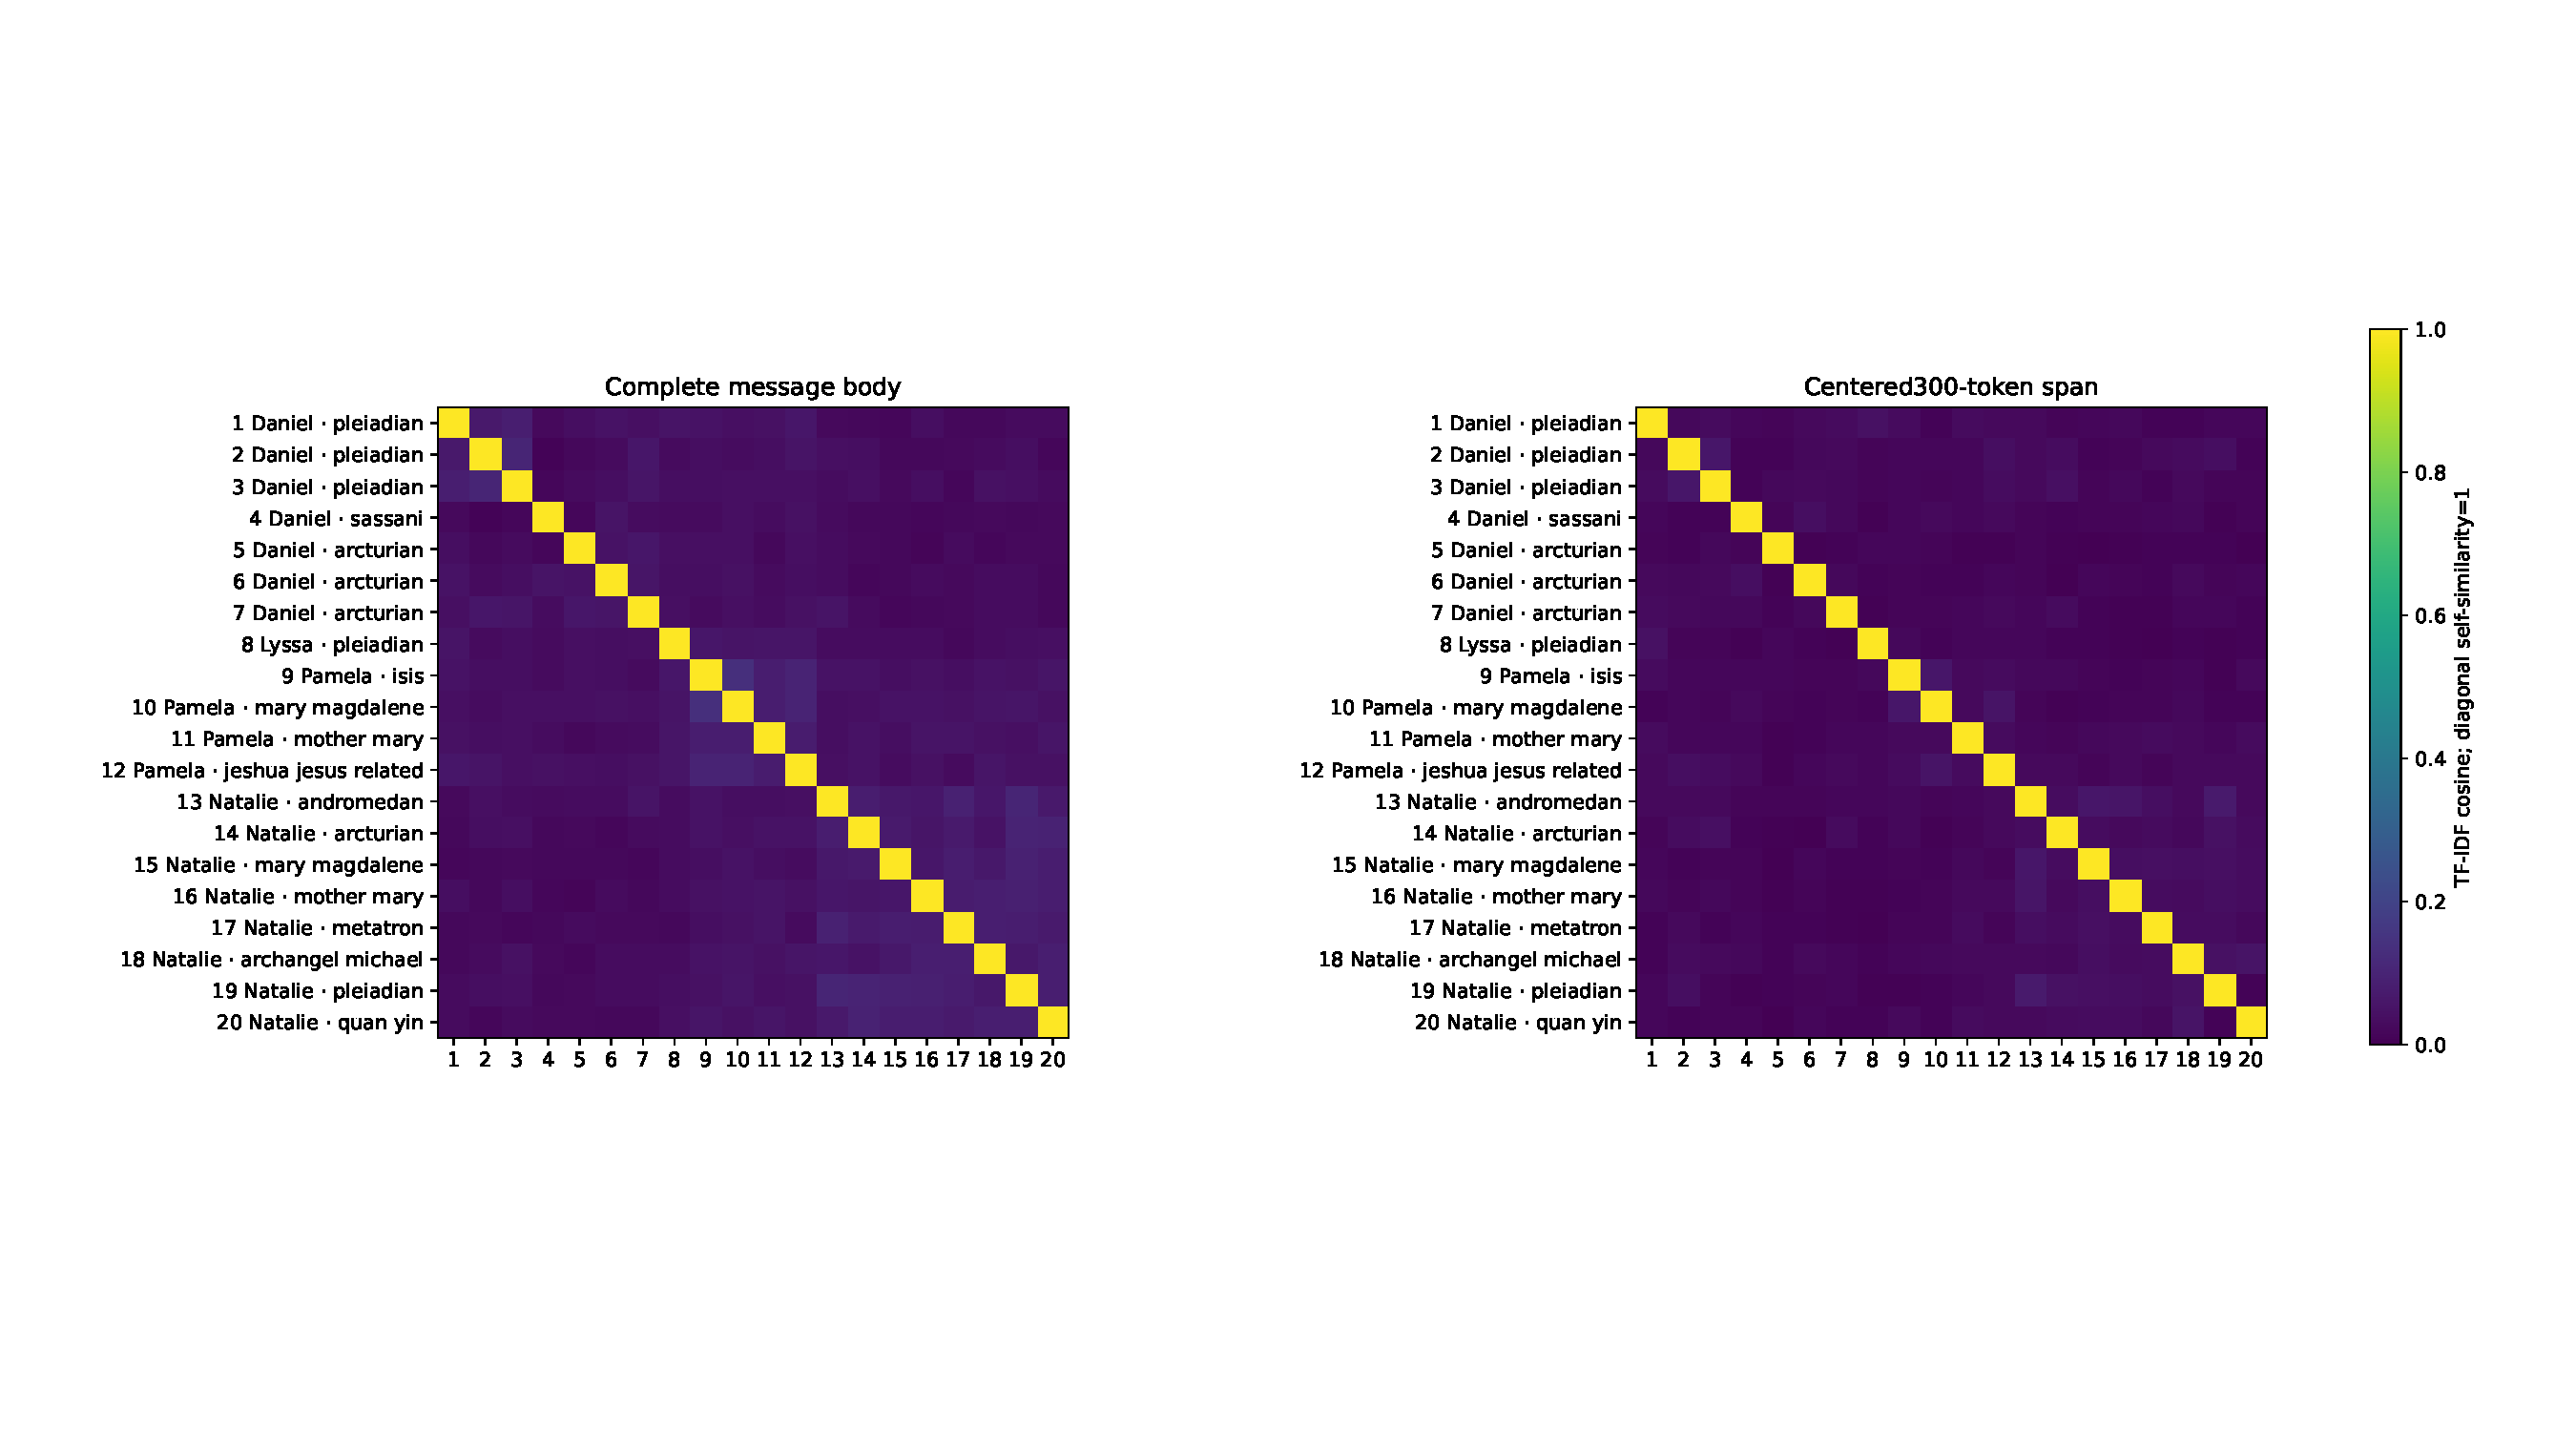
\includegraphics[width=1\textwidth,height=\textheight]{figures/pilot-similarity.pdf}
\caption{Pilot pairwise similarities with their source-specific document
ordering. This matrix belongs to the 20-message fit and must not be
numerically merged with the separately fitted 292-unit matrix.}
\end{figure}

The initial partial name-token mask left council-title phrases such as
\emph{high council} and \emph{council seven}. A targeted sensitivity
removed the full Pleiadian High Council and Arcturian Council title
patterns, plus the specified Seven Pleiadians expression. Shared-label
cross-medium mean cosine changed from \textbf{0.03636 to 0.03648}, while
different-label within-medium mean changed from \textbf{0.06588 to
0.06538}. The maximum individual pair change was \textbf{0.03483}.
Stable group averages can therefore coexist with noticeable movement in
an individual pair. This test addresses the declared phrases; it does
not prove the absence of other source signatures.

\begin{figure}
\centering
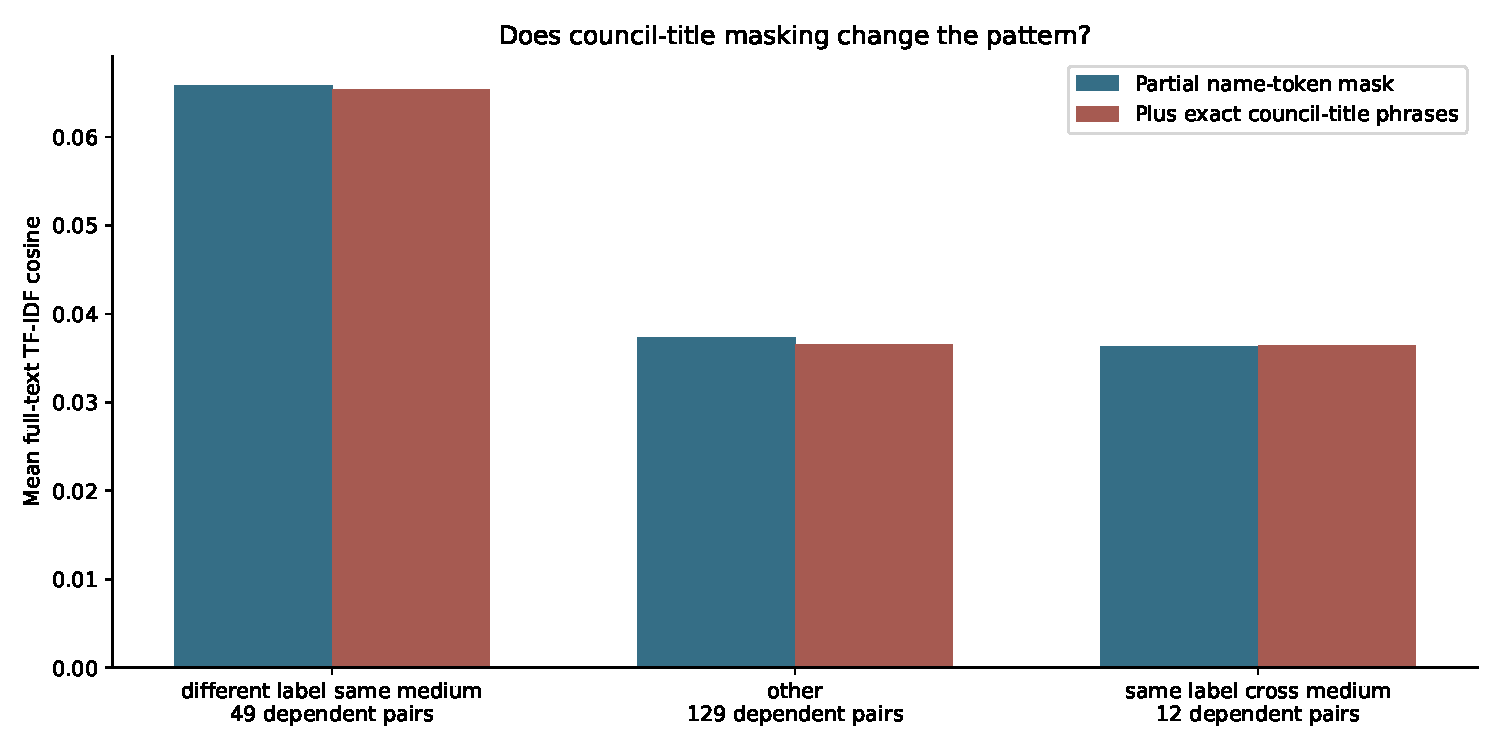
\includegraphics[width=1\textwidth,height=\textheight]{figures/pilot-title-sensitivity.pdf}
\caption{Council-title masking sensitivity. The direction of the
descriptive group contrast persists under this specific refit, without
supplying a significance test or eliminating selection and provenance
confounding.}
\end{figure}

The pilot's declared three-cluster display has silhouette
\textbf{0.02774}, source-medium adjusted Rand index \textbf{0.61778} and
mean seed-pair adjusted Rand agreement \textbf{0.83769}. These modest
separation and source-alignment diagnostics support cautious exploratory
use. They do not validate a three-topic account of the eleven comparison
labels.

\FloatBarrier

\subsection{Source reading separates themes from
recommendations}\label{source-reading-separates-themes-from-recommendations}

The Mother Mary messages share language about inward care, love and joy,
yet their practical emphases differ.\footnote{Publisher message bodies:
  \href{https://omna.org/do-you-trust-the-universe-by-mother-mary/}{Glasson
  / Mother Mary} and
  \href{https://www.jeshua.net/channelings/mother-mary/high-sensitivity/}{Kribbe
  / Mother Mary}. Page-local attribution and body boundaries are
  recorded in the pilot.} The Glasson message frames distrust through
disconnection from inner love and a generous universe. The Kribbe
message emphasizes inner-child care, emotional boundaries and, where
appropriate, leaving a draining situation. It would be an overreading to
turn the former into a universal claim that every adverse circumstance
is merely internal, or to omit the latter's permission to change an
external situation. The two bodies were also independently read by the
critic, totaling 2,216 words. Their comparison does not show that one
observed question was answered twice, and it does not authenticate a
sacred speaker.

The Magdalene pair illustrates a related distinction.\footnote{Publisher
  message bodies:
  \href{https://omna.org/grace-embrace-initiation-by-mary-magdalene/}{Glasson
  / Mary Magdalene} and
  \href{https://www.jeshua.net/channelings/mary-magdalene/the-fire-in-your-belly/}{Kribbe
  / Mary Magdalene}.} One message centers on grace, initiation and an
imagined embrace extending to surrounding circumstances. The other
centers on embodied passion, shadow feelings and the integration of
heart and bodily desire, together with a source-claimed autobiographical
narrative about gender and religion. A keyword cluster could group both
as inward transformation while missing their different frameworks. The
latter also qualifies its discussion by acknowledging potentially
dominating or manipulative expressions of energy; omitting that
qualification would overstate its practical endorsement.

The Pleiadian comparison spans a named High Council, an unnamed
collective and Sasha.\footnote{Publisher sources:
  \href{https://danielscranton.com/introductions-pleiadian-high-council/}{Scranton
  / High Council introduction},
  \href{https://omna.org/recentering-your-ascension-by-pleiadians/}{Glasson
  / Pleiadians}, and
  \href{https://www.lyssaroyal.net/uploads/1/5/7/1/15716170/tran-preparedness138.pdf}{Royal
  / Sasha, Preparedness excerpt}. These are three different
  source-specific speaker labels within a broad comparison group.} The
selected Scranton message rejects a universal formula and emphasizes
choice, intuition and community. The Glasson message recommends daily
recentering and reducing spiritual distraction. Sasha's excerpt
discusses debt, tangible wealth, self-responsibility and an imagined
Equal Value System. Its communal model is expressly distinguished from
hoarding and presented as one society's example. These are different
source recommendations across different eras and genres, not a single
Pleiadian doctrine. The financial material is analyzed as published
discourse, not endorsed as investment advice or evaluated economics.

The Arcturian comparison likewise contrasts a purported history of
bodily, nature-based and meditative practices with a present-focused
attention exercise.\footnote{Publisher message bodies:
  \href{https://danielscranton.com/ancient-arcturian-practices-\%e2\%88\%9ethe-9d-arcturian-council/}{Scranton
  / Arcturian Council practices} and
  \href{https://omna.org/as-you-focus-so-you-become-by-the-arcturians/}{Glasson
  / Arcturians attention exercise}.} Both encourage inward awareness and
personal resonance, but the form of their explanation differs. The
attention message permits anger or low feelings as part of a process;
summarizing it as an obligation to remain positive would omit a material
qualification. None of these readings establishes the historical society
or mechanism described by the source.

\FloatBarrier

\subsection{The sole surviving question lead is not an equivalent
question}\label{the-sole-surviving-question-lead-is-not-an-equivalent-question}

Of 2,629 unverified punctuation candidates, \textbf{411} meet the
eligibility conditions; \textbf{1,949} Ra questions are eligible
targets. The corrected retrieval abstains on \textbf{410} candidates and
forwards one lead for reading. Its cosine is \textbf{0.40289}, with a
runner-up gap of \textbf{0.14576}, so it clears the declared heuristic
thresholds.

The source reading nevertheless rejects it. An interview fragment asks
whether the present era differs from a thousand years earlier. The
matched Ra passage, printed question 16.14, asks for the name of an
ancient visitor. Shared time-span wording conceals different information
needs. The interview candidate has no identified answer; the Ra answer
is a documentary attribution. The result is \textbf{zero accepted
same-question pairs and zero identified non-Ra answers} from this
retrieval pass.

At otherwise unchanged settings, cosine thresholds of 0.25, 0.35, 0.45
and 0.55 yield two, one, zero and zero leads respectively. Those counts
are a sensitivity display, not a precision-recall evaluation. The false
match demonstrates a practical limit: retrieval can propose a source for
review, but lexical resemblance alone cannot supply a valid cross-medium
question-and-answer comparison.

\FloatBarrier

\section{Dashboard, review and
reproducibility}\label{dashboard-review-and-reproducibility}

The dashboard exposes the claim network, comparison matrix, source
records, collection status, joint analysis and separate pilot. The
interface distinguishes direct attribution from weaker links, and it
gives source-level access to the evidence behind a group. Missing
transcript coverage is labeled as insufficient observed cross-medium
text rather than plotted as zero similarity. Topic summaries refer to
factors, and the Q/A card marks the inspected candidate as rejected
rather than an accepted match.

Two substantive rounds of model-agent work are recorded. The five roles
covered source research across ET and religious/named-person material,
quantitative methods, interface design, and independent criticism. These
are AI work roles, not five human subject experts. The first round
established concrete evidence and acquisition requirements. The second
inspected actual source passages, normalized text, numerical outputs and
interface behavior, then recorded corrections.

Those corrections included the Andrew training attribution,
source-private-path removal, role normalization, preservation of
category-only evidence, exclusion of comments from publisher assertions,
response-only handling of the Lyssa dialogue, a missing cross-register
group membership, and the council-title sensitivity. A visual review
also repaired a colorbar overlap without changing the joint numerical
results. The critic independently recomputed 98 joint full/window group
cells, all 411 eligible retrieval decisions, 800 pilot full/window
cells, all 190 pilot pair scores/classifications, and the 400-cell
council-title sensitivity. NMF and KMeans were not independently
refitted by the critic.

Interface receipts document 199 network checks and 967 subscription
checks, together with screenshots and CSV exports. They address
navigation, filtering, keyboard interaction, legibility and runtime
errors. They do not verify the truth of the corpus's source claims. A
source-review subset and the nine-body interpretive reading remain
explicitly bounded rather than being described as full human annotation.

This paper pins the final joint, pilot and graph artifacts in
\texttt{snapshot.json}. The joint final-02 hash is
\texttt{34ac7bbe...e7a6722}; the pilot final-02 hash is
\texttt{2fd5c744...cc2d8b6}. Complete hashes and upstream inputs are
supplied with the artifact, along with figure files, Markdown, LaTeX,
bibliography, a portable build script and a generated build manifest.
Rebuilding the paper from those provided public inputs is distinct from
refitting models, which requires the separately retained permitted
private corpus. Ongoing audio and ASR processing are not silently added
to the frozen model inputs.

\FloatBarrier

\section{Limitations and responsible
interpretation}\label{limitations-and-responsible-interpretation}

\textbf{Selection and missingness.} Accessible publishers and
user-selected leads shape the source frame. Search rankings, current
feed windows, public excerpts, language availability and access failures
all influence inclusion. The source register is broader than the fitted
corpus, and the 20-message pilot covers only four mediums. Its periods
range from a 1993 excerpt to recent publisher messages. A completed
collection of a declared frame would still not establish an exhaustive
history of every channel or an unbiased sample of all traditions.

\textbf{Attribution and dependence.} A publisher's naming is an
observable assertion, not authenticated identity. Shared labels do not
establish a shared speaker, and distinct mediums do not prove
independent origin. Joint practices, self-described training lineages,
reposts and source families matter. Exact duplicate checks address exact
aliases; they do not resolve all paraphrase, excerpt, edition or
recording lineage. A series listing or category name cannot stand in for
a reviewed message.

\textbf{Language, editing and ASR.} The text collections combine
editorial and production processes. Translation, prepared writing,
question structure, caption segmentation and recognition error can shape
lexical patterns. The 20-body pilot has page-local attribution but no
verified audio alignment. The response-only PDF derivative depends on
printed layout. No measured ASR error rate, hallucination rate,
diarization accuracy or human inter-annotator reliability is available
for these analyses.

\textbf{Construct validity.} TF-IDF cosine measures overlap in weighted
lexical features. It does not directly measure agreement, contradiction,
identity, cultural equivalence or the practical quality of advice. Topic
factors and clusters may recover source signatures. The pair averages
use dependent observations and unequal label coverage. No inferential
significance test, causal estimate, external classifier validation or
quantitative supernatural probability is claimed.

\textbf{Interpretation and representation.} The close readings are
model-assisted and purposive. They preserve bounded differences and
counterexamples, but they are not a substitute for expert religious
scholarship, human qualitative coding or representative audience
research. Contemporary messages using names from religious traditions do
not become official or typical doctrine. Text concerning finance, health
or other consequential topics is source content under analysis, not a
validated recommendation.

\textbf{Release and storage.} Public accessibility does not provide
blanket permission to republish full books, transcripts or recordings.
The public artifacts therefore contain code, metadata, derived values
and limited paraphrases. Full source material and detailed Q/A fragments
remain in private storage under their recorded collection basis. A
managed workspace is not represented as permanent account-wide ChatGPT
storage. Downloaded original bytes, retained converted audio, completed
transcripts and analyzed units remain separate operational categories.

\FloatBarrier

\section{Next experiments}\label{next-experiments}

A useful next phase should improve comparability before increasing model
complexity. A prospectively specified sampling design could select
multiple dated messages per directly attributed label and medium,
balance message length and genre, and retain source-family identifiers
across editions and clips. Human reviewers could then annotate a
stratified set of speaker roles, practical recommendations, source
references and actual question equivalence, with an abstention category
and a held-out disagreement audit. These tasks are \textbf{TBD}, not
completed validation.

A matched-message design could distinguish broad civilization labels
from the same written name and compare within-medium and cross-medium
contrasts while controlling the sampling frame more explicitly. Repeated
or translated texts should be identified before any uncertainty
calculation. A resampling or hierarchical model would require a
defensible independent sampling unit; the current pair count should not
be treated as that unit. Future topic-model comparisons could test
whether judgments survive alternative representations, source masking
and human document-level interpretation.

For recordings, a listening audit should precede inference about
fine-grained statements. It should cover poor-quality historical audio,
short clips, silence, multiple speakers and representative accents or
languages, binding every assessed excerpt to actual audio. Q/A work
should first establish real prompts and responses within a recording,
then test cross-source equivalence. Only after those steps would it be
meaningful to evaluate a retrieval-augmented assistant or a fine-tuned
model on held-out source-grounded tasks. No new fine-tuned model or
inference improvement is claimed by this paper.

\FloatBarrier

\section{Conclusion}\label{conclusion}

This expansion makes comparison possible by preserving differences that
a large undifferentiated archive would hide. The typed register
identifies repeated labels, while the text layer shows how little of
that larger map is currently covered by comparable messages. The joint
corpus organizes strongly by source context. The new pilot exhibits
greater lexical overlap within mediums across labels than across mediums
sharing a label, and that descriptive contrast persists under the
specified council-title sensitivity. Its selection and provenance
prevent a causal or identity conclusion. The rejected Q/A lead further
demonstrates why a retrieval score must remain a prompt for source
reading. The resulting living paper and dashboard support additional
collection and criticism without turning missing text, shared names or
attractive plots into evidence they cannot supply.

\clearpage

\section{References}\label{references}

\phantomsection\label{refs}
\begin{CSLReferences}{1}{0}
\bibitem[\citeproctext]{ref-bender2018}
Bender, Emily M., and Batya Friedman. 2018. {``Data Statements for
Natural Language Processing: Toward Mitigating System Bias and Enabling
Better Science.''} \emph{Transactions of the Association for
Computational Linguistics} 6: 587--604.
\url{https://doi.org/10.1162/tacl_a_00041}.

\bibitem[\citeproctext]{ref-doogan2021}
Doogan, Caitlin, and Wray Buntine. 2021. {``Topic Model or Topic
Twaddle? Re-Evaluating Semantic Interpretability Measures.''} In
\emph{Proceedings of the 2021 Conference of the North American Chapter
of the Association for Computational Linguistics: Human Language
Technologies}, 3824--48.
\url{https://doi.org/10.18653/v1/2021.naacl-main.300}.

\bibitem[\citeproctext]{ref-kapoor2023}
Kapoor, Sayash, and Arvind Narayanan. 2023. {``Leakage and the
Reproducibility Crisis in Machine-Learning-Based Science.''}
\emph{Patterns} 4 (9): 100804.
\url{https://doi.org/10.1016/j.patter.2023.100804}.

\bibitem[\citeproctext]{ref-koenecke2024}
Koenecke, Allison, Anna Seo Gyeong Choi, Katelyn X. Mei, Hilke
Schellmann, and Mona Sloane. 2024. {``Careless Whisper: Speech-to-Text
Hallucination Harms.''} In \emph{The 2024 ACM Conference on Fairness,
Accountability, and Transparency}, 1672--81.
\url{https://doi.org/10.1145/3630106.3658996}.

\bibitem[\citeproctext]{ref-schroeder2025}
Schroeder, Kayla, and Zach Wood-Doughty. 2025. {``Reliability of Topic
Modeling.''} In \emph{Proceedings of the 2025 Conference of the Nations
of the Americas Chapter of the Association for Computational
Linguistics: Human Language Technologies}, 2649--62.
\url{https://doi.org/10.18653/v1/2025.naacl-long.134}.

\end{CSLReferences}

\clearpage

\section{Appendix A: reference access and
reuse}\label{appendix-a-reference-access-and-reuse}

The following reading depths come from the earlier methodological-source
ledger. They are reused here, not reported as new full-paper reading.

\begin{longtable}[]{@{}
  >{\raggedright\arraybackslash}p{(\columnwidth - 4\tabcolsep) * \real{0.2500}}
  >{\raggedright\arraybackslash}p{(\columnwidth - 4\tabcolsep) * \real{0.3600}}
  >{\raggedright\arraybackslash}p{(\columnwidth - 4\tabcolsep) * \real{0.3900}}@{}}
\toprule\noalign{}
\begin{minipage}[b]{\linewidth}\raggedright
Reference
\end{minipage} & \begin{minipage}[b]{\linewidth}\raggedright
Recorded access
\end{minipage} & \begin{minipage}[b]{\linewidth}\raggedright
Limit on use here
\end{minipage} \\
\midrule\noalign{}
\endhead
\bottomrule\noalign{}
\endlastfoot
Doogan and Buntine (2021) & Official 25-page PDF retrieved; pages 1, 4,
6 and 9 inspected. & Supports caution about interpretability measures;
its human expert evaluation was not replicated. \\
Schroeder and Wood-Doughty (2025) & Official 14-page PDF retrieved;
pages 1, 2 and 9 inspected. & LDA study; it does not validate NMF
reliability or a cosine threshold. \\
Bender and Friedman (2018) & Official 18-page PDF retrieved; pages 1, 4
and 5 inspected. & Supports data-statement reporting; it does not
establish causal comparability of these source contexts. \\
Kapoor and Narayanan (2023) & Published metadata checked; complete
author-preprint abstract v1 read. & Full taxonomy and paper body were
not inspected in that increment. \\
Koenecke et al.~(2024) & Published metadata checked; complete
author-preprint abstract v2 read. & Publisher PDF was unavailable; its
error rates and conditions are not transferred to this study. \\
\end{longtable}

\clearpage

\section{Appendix B: complete comparison
coverage}\label{appendix-b-complete-comparison-coverage}

\begin{longtable}[]{@{}
  >{\raggedright\arraybackslash}p{(\columnwidth - 8\tabcolsep) * \real{0.4000}}
  >{\raggedright\arraybackslash}p{(\columnwidth - 8\tabcolsep) * \real{0.1500}}
  >{\raggedright\arraybackslash}p{(\columnwidth - 8\tabcolsep) * \real{0.1500}}
  >{\raggedright\arraybackslash}p{(\columnwidth - 8\tabcolsep) * \real{0.1500}}
  >{\raggedright\arraybackslash}p{(\columnwidth - 8\tabcolsep) * \real{0.1500}}@{}}
\caption{Complete frozen comparison-group coverage. Direct/practice
counts describe attributed records, not verified ability or independent
origin. Pilot documents and mediums refer only to the separately fitted
20-message cohort; zero denotes absent admitted pilot text. The Ra and
Bashar historical joint corpus remains available under its own
source-context grain.}\tabularnewline
\toprule\noalign{}
\begin{minipage}[b]{\linewidth}\raggedright
Group
\end{minipage} & \begin{minipage}[b]{\linewidth}\raggedright
Direct people
\end{minipage} & \begin{minipage}[b]{\linewidth}\raggedright
Declared practices
\end{minipage} & \begin{minipage}[b]{\linewidth}\raggedright
Pilot texts
\end{minipage} & \begin{minipage}[b]{\linewidth}\raggedright
Pilot mediums
\end{minipage} \\
\midrule\noalign{}
\endfirsthead
\toprule\noalign{}
\begin{minipage}[b]{\linewidth}\raggedright
Group
\end{minipage} & \begin{minipage}[b]{\linewidth}\raggedright
Direct people
\end{minipage} & \begin{minipage}[b]{\linewidth}\raggedright
Declared practices
\end{minipage} & \begin{minipage}[b]{\linewidth}\raggedright
Pilot texts
\end{minipage} & \begin{minipage}[b]{\linewidth}\raggedright
Pilot mediums
\end{minipage} \\
\midrule\noalign{}
\endhead
\bottomrule\noalign{}
\endlastfoot
Pleiadian labels & 11 & 10 & 5 & 3 \\
Arcturian labels & 2 & 2 & 4 & 2 \\
Yahyel labels & 2 & 2 & 0 & 0 \\
Zeta labels & 1 & 1 & 0 & 0 \\
Bashar & 2 & 2 & 0 & 0 \\
Sassani / Essassani vocabulary & 3 & 3 & 1 & 1 \\
Ra / RA & 1 & 1 & 0 & 0 \\
Kryon & 1 & 1 & 0 & 0 \\
Andromedan labels & 1 & 1 & 1 & 1 \\
Archangel Michael & 4 & 4 & 1 & 1 \\
Archangel Gabriel & 2 & 2 & 0 & 0 \\
Mother Mary & 2 & 2 & 2 & 2 \\
Mary Magdalene / Magdalen & 3 & 3 & 2 & 2 \\
Jeshua / Yeshua / Jesus-related & 2 & 2 & 1 & 1 \\
Saint Germain / Adamus Saint-Germain & 3 & 3 & 0 & 0 \\
Quan Yin & 2 & 2 & 1 & 1 \\
The Hathors & 2 & 2 & 0 & 0 \\
Erik Medhus & 1 & 1 & 0 & 0 \\
Krishna & 1 & 1 & 0 & 0 \\
\end{longtable}

\clearpage

\section{Appendix C: artifact and review
boundaries}\label{appendix-c-artifact-and-review-boundaries}

The public inputs under the channeling-network dashboard are:

\begin{itemize}
\tightlist
\item
  \texttt{analysis.json}: accepted joint analysis.
\item
  \texttt{new-message-pilot.json}: separate attributed-message pilot.
\item
  \texttt{claim-graph-statistics.json}: typed graph and comparison
  coverage.
\item
  \texttt{et-register.json}: ET source and attribution register.
\item
  \texttt{traditions-register.json}: religious and named-person source
  register.
\end{itemize}

The paper snapshot stores their complete hashes and the specific
method/review documents used. The existing Bashar--Ra paper remains a
separate artifact and was not edited for this companion.

The new paper figures either copy the accepted vector/raster outputs
unchanged or render the typed source and coverage data from the frozen
snapshot. The rebuild script compiles the supplied Markdown and
bibliography into LaTeX and PDF, then hashes the local public artifact
set. Optional figure regeneration uses \texttt{plot\_snapshot.py}; it
performs no topic fitting or corpus analysis. Model refitting, media
acquisition, ASR recognition and paper compilation are different
operations with different prerequisites and should not be conflated in a
reproducibility claim.

\end{document}
